\chapter{Building a corpus for event detection on Twitter}

\section{Introduction}

Research on social media topic detection and tracking (without specification
of the type of topic) lacks some publicly available tweet
datasets to produce reproducible results. This is all the
more true for non-English languages. Some datasets exist, but they often have different definitions of event or topic than ours: many works on event detection are actually focused on  burst detection (detecting topics such as natural disasters, attacks, etc., that cause an unusual volume of tweets) and do not attempt to assess the relative size of events. 
Therefore, we needed to build our own evaluation corpus that would fit our needs in term of language (French), representativity of the collected tweets, quality and diversity of the annotated events. This introduction details the properties expected from such a corpus. In the rest of the chapter, we present the existing Twitter events datasets, then we detail our tweet collection method and our annotation process. Finally, we propose several ways of evaluating the created corpus.

\subsection{Representativity of the collected data}
In an ideal world, to compare news production on social media and on mainstream media, one would need the universe – during a given period of time (e.g. the year 2018) and a geographical location (e.g. France, the UK or the US) – of all documents published on the one hand on social media and on the other hand on mainstream media. Unfortunately, given the limitation of the Twitter API, it is not possible for the researcher to capture the universe of the documents (or tweets) published on Twitter. However, the researcher can work on a sample of the documents, as long as this sample is ``representative”. Why do we need representativity?


Assume that we get access to a subsample of the documents published on Twitter, but that this sample is not representative of the overall traffic. For example, assume that this sample of tweets is such that the tweets’ characteristics (perhaps because the API provides the researcher with documents tweeted by users with more followers) are such that these documents have a higher probability to make it to the mainstream media. Then using this biased subsample will lead the researcher to overestimate the probability for a news story broken on social media to appear on mainstream media.


The same issue will arise if the researcher wants to tackle the follow-up question: what are the determinants of the success of a news story initially broken on social media? Imagine that the researcher is using a selected sample of tweets that is not representative. Imagine for example that this sample of tweets comes mainly from journalists working for a given media, e.g. \textit{Le Monde}, and that, at the same time, within the set of tweets posted by \textit{Le Monde}’s journalists, only the successful ones are part of the sample, then the results of the empirical analysis will be biased in favor of \textit{Le Monde}. In other words, when the researcher will study the impact of the company for which the journalist works (independent variable) on the probability for the news story broken on Twitter to make it to mainstream media (dependent variable), the coefficient obtained for \textit{Le Monde} will ovestimate the real causal impact of the company.


It seems very difficult to correct for this kind of biases. Hence the necessity to have a representative sample of tweets, i.e. a sample of tweets such that the tweets included in our sample do not differ from the tweets that are not included along all the dimensions that may have a direct impact on the dependent variable of interest.

\subsection{Quality of the annotated events}

The properties of a given corpus have an impact on the implementation of the detection algorithm: for example, if all events in our corpus tend to grow at a high rate (\textit{i.e.} people react very quickly to that event on social media), a simple way to increase the performance of our program would be to select group of tweets that have a high growth rate and discard others as ``non events". However, this would result in a program unable to detect other types of events and introduce bias in our results. Therefore, the choices made during the creation of the annotated corpus are critical to ensure that our program can detect a large variety of events.

The size of events is also an important parameter that needs to be taken into account: small events, that generate few tweets, are difficult to detect automatically and this is precisely why they need to be represented in our test corpus. On the other hand, large events, like the 2018 FIFA World Cup, generate so many tweets that it is impossible to annotate all of them manually. This is an inevitable flaw in any manually annotated corpus. We take this flaw into account when evaluating the event detection algorithm  \textbf{\color{orange}(see Section?).}

It is also necessary to ensure the diversity of events in the corpus in terms of subject (sport, economy, science and technology, etc.) and regarding the origin of events (events having emerged on Twitter vs. events first covered by news media). The diversity of tweets inside each annotated event is also an important matter: ideally, tweets should originate from a variety of sources, and not be written only by journalists or media accounts.

The following section details the choices made by the authors of existing datasets with regard to these quality criteria.
        
		
%		\paragraph{\textbf{Categories}}
%		\citet{mcminn_building_2013} test the diversity of their corpus by examining the events' distribution across 8 categories. These categories where created from a mapping between TDT categories \citep{allan_introduction_2002} and Wikipedia categories. They identify differences in the distribution depending on the event selection method : for example, approaches based on pre-detection produce more clusters about ``Sport" and less about ``Armed Conflicts and Attacks" than the Wikipedia-based approach. It is likely that sports events are more discussed on Twitter than by traditional news media which would explain why they were not selected as ``events" by the Wikipedia community.


\section{State of the art: event detection corpora}
\label{state of the art}
Twitter gives a limited access to its data, but still provides some API endpoints to retrieve tweets (which is not the case of other more popular social networks), hence the large number of works based on Twitter datasets. However, few of them provide access to their evaluation corpora. We detail available event detection collections in this section.

\citet{mcminn_building_2013} created the largest available corpus on event detection. They used several methods to generate candidate events: two automatic event detection methods on their set of 120 million tweets in English and one method based on query expansion of Wikipedia events. The automatically generated events were then assessed using Amazon Mechanical Turk, firstly to evaluate if the automatically generated events corresponded to their definition of event, secondly to judge if the clustered tweets where all relevant to the event. They finally merged together the events from the three candidate generation methods and removed duplicate events. The final corpus consists in more than 100,000 annotated tweets covering 506 events. However, this corpus dates from 2012. Because of tweets beeing removed and Twitter accounts being closed, a large part of this dataset can no longer be recovered. In August 2018, we could only retrieve 66.5 million tweets from the original collection (55\%) and 72,790 tweets from  the annotated corpus (72\%).

The SNOW dataset \citep{papadopoulos_snow_2014} can also be used as test corpus for an event detection task. It is composed of 59 events from the headlines of the BBC RSS newsfeed and from NewsWhip UK published during one day (25 Feb. 2014). However it does not provide comprehensive sets of tweets related to each event, only two to five “representative” tweets from a collection of more than 1 million tweets emitted on that date.

The \textit{Text REtrieval Conference} (TREC) microblog datasets where released in 2014 \cite{lin2014overview} and 2015 \cite{lin2015overview}. The most recent consists of more than 60,000 tweets posted between July 19, 2015, and July 30, 2015, annotated in relationship with one of 51 topics. These tweets were sent by participants in response to the Microblog TREC tasks, that comprise two scenarios: (a) a "push notification" system returns tweets considered as "interesting and novel" to a user having defined a topic of interest, and (b) a daily "email digest" is sent to a user with tweets containing relevant updates concerning her topic of interest. The 51 interest profiles cannot exactly be defined as "events", but rather general themes, such as for example "Find information about the possibility of the passage of gay marriage laws in Europe.", or "Find information about bridge tournaments in the United States in July or August 2015.". The tweets sent by participants to the task where then annotated by assessors as "relevant", "not relevant" or "highly relevant". This dataset is an interesting resource for our task, but a little less relevant than that of \citet{mcminn_building_2013}, because the annotated tweets have been selected for their "novelty": the dataset therefore includes many tweets announcing "breaking news", and few tweets of conversation or opinion on topics already known.

The datasets from the 2013 and 2014 MediaEval Social Event Detection tasks \cite{reuter2013social, petkos2014social}, are also important corpora to test event detection systems, and multimodal systems in particular. The first challenge of this task consists in clustering images of social events so that each cluster matches an event. The events correspond to sport events, protest marches, BBQs, debates, expositions, festivals or concerts all registered on the last.fm database. The authors downloaded pictures tagged with the last.fm event ids on Flickr. In total, each dataset contains 300,000 training images from approximately 20,000 events. This corpus is very interesting because of its size and the large number of different events it contains. However, the fact that it contains only "social events" (public gathering attended by a large number of people) restricts the task to a certain type of subjects. The type of images shared on Flickr is also very different from those shared on Twitter: they are mostly photos taken by users themselves, with few duplicate images. Conversely, images on Twitter are very often re-used by several users, sometimes in different contexts, which makes the task more complex. 

The Signal-1M corpora consist on a dataset of 1 million news articles from September 2015 \citep{corney2016million}, and of a dataset of tweets related to 100 randomly selected articles \citep{suarez2018data}. The tweets dataset contains approximatively 6000 tweets.

The News Event Dataset \citep{mele2019multi} contains 147,000 documents from 9 news channels and published on Twitter, RSS portals and news websites from March to June 2016. 57 media events were annotated on a crowdsourcing platform, to label 4300 documents, including 744 tweets.

The last two datasets contain too few tweets to allow a large-scale evaluation of any event detection and tracking system. In addition, events in SNOW, Signal-1M and the News Events Dataset are selected from media sources only. Only the corpus by \citet{mcminn_building_2013} relies on a topic detection step among collected tweets before proceeding to the annotation step. This method allows for a greater variety of events, but it is likely to influence the evaluation: indeed, event detection systems similar to those used by \citet{mcminn_building_2013} for corpus creation may get better results when tested on this corpus.

We tried to avoid these biases when creating our own corpus. The methodology used to build our dataset is detailed in the two following sections.

\section{Tweet collection}
\label{Tweet collection}
Our objective is to collect automatically and continuously a set of tweets representative to the real Twitter activity. In addition to being \textbf{representative}, this corpus must contain a \textbf{volume of tweets sufficient for media events to be represented} in it, in particular medium and small events. Besides, these tweets must be \textbf{in French}. The following sections present the methods used to achieve these objectives.
\subsection{Constraints}
Their are different ways of collecting large volumes of tweets, although collecting the full volume of tweets emitted during a given period is not possible. Indeed, even if Twitter is known for providing a larger access to its data than other social media platforms,\footnote{In particular, despite the research effort recently launched by Facebook, it is still nearly impossible for researchers outside Facebook to get access to information on users' activity on the platform.} the Twitter streaming APIs are strictly limited in term of volume of returned tweets. These limitations are all constraints that we must integrate into our collection procedure.
	
	


\paragraph{Sample API:}

the Sample API\footnote{\url{https://developer.twitter.com/en/docs/tweets/sample-realtime/overview/get_statuses_sample}} continuously provides 1\% of the tweets posted around the world at a given moment. Once connected to the API at time $t_0$, the user gets 1\% of all tweets emitted after $t_0$, and receives regular batches of tweets as long as she stays connected. Twitter provides little information on how the sample is generated. However,  \citet{kergl_endogenesis_2014} have studied it by analyzing the ids of tweets (based on a timestamp in milliseconds and on a number of series to identify tweets issued during the same millisecond). They show that all tweets provided by the API were issued between the 657th and 666th milliseconds of each second, which should assure the user to receive a constant stream representing around 1\% of the total. Another study done on the distribution of tweets in the Sample API in comparison with another paid API, which provides full access to all emitted tweets, shows no statistically significant difference between the two samples \citep{morstatter_when_2014}.


This API does not meet our needs, since the proportion of tweets in French is only 1.8\% of the total sample on average (Figure \ref{Figure:HistogramLanguages} illustrate the distribution of tweets in different languages). Moreover, according to \citet{liu_reuters_2016}, the proportion of tweets concerning news is less than 0.2\%. If we combine all these restrictions, we could only have access to 92,000 tweets in French a day, and less than 200 tweets a day concerning news if we were to simply use the Sample API provided by Twitter.

%%%%%%%%%%%%%%%%%%%%%%%%
\begin{figure}
\begin{center}
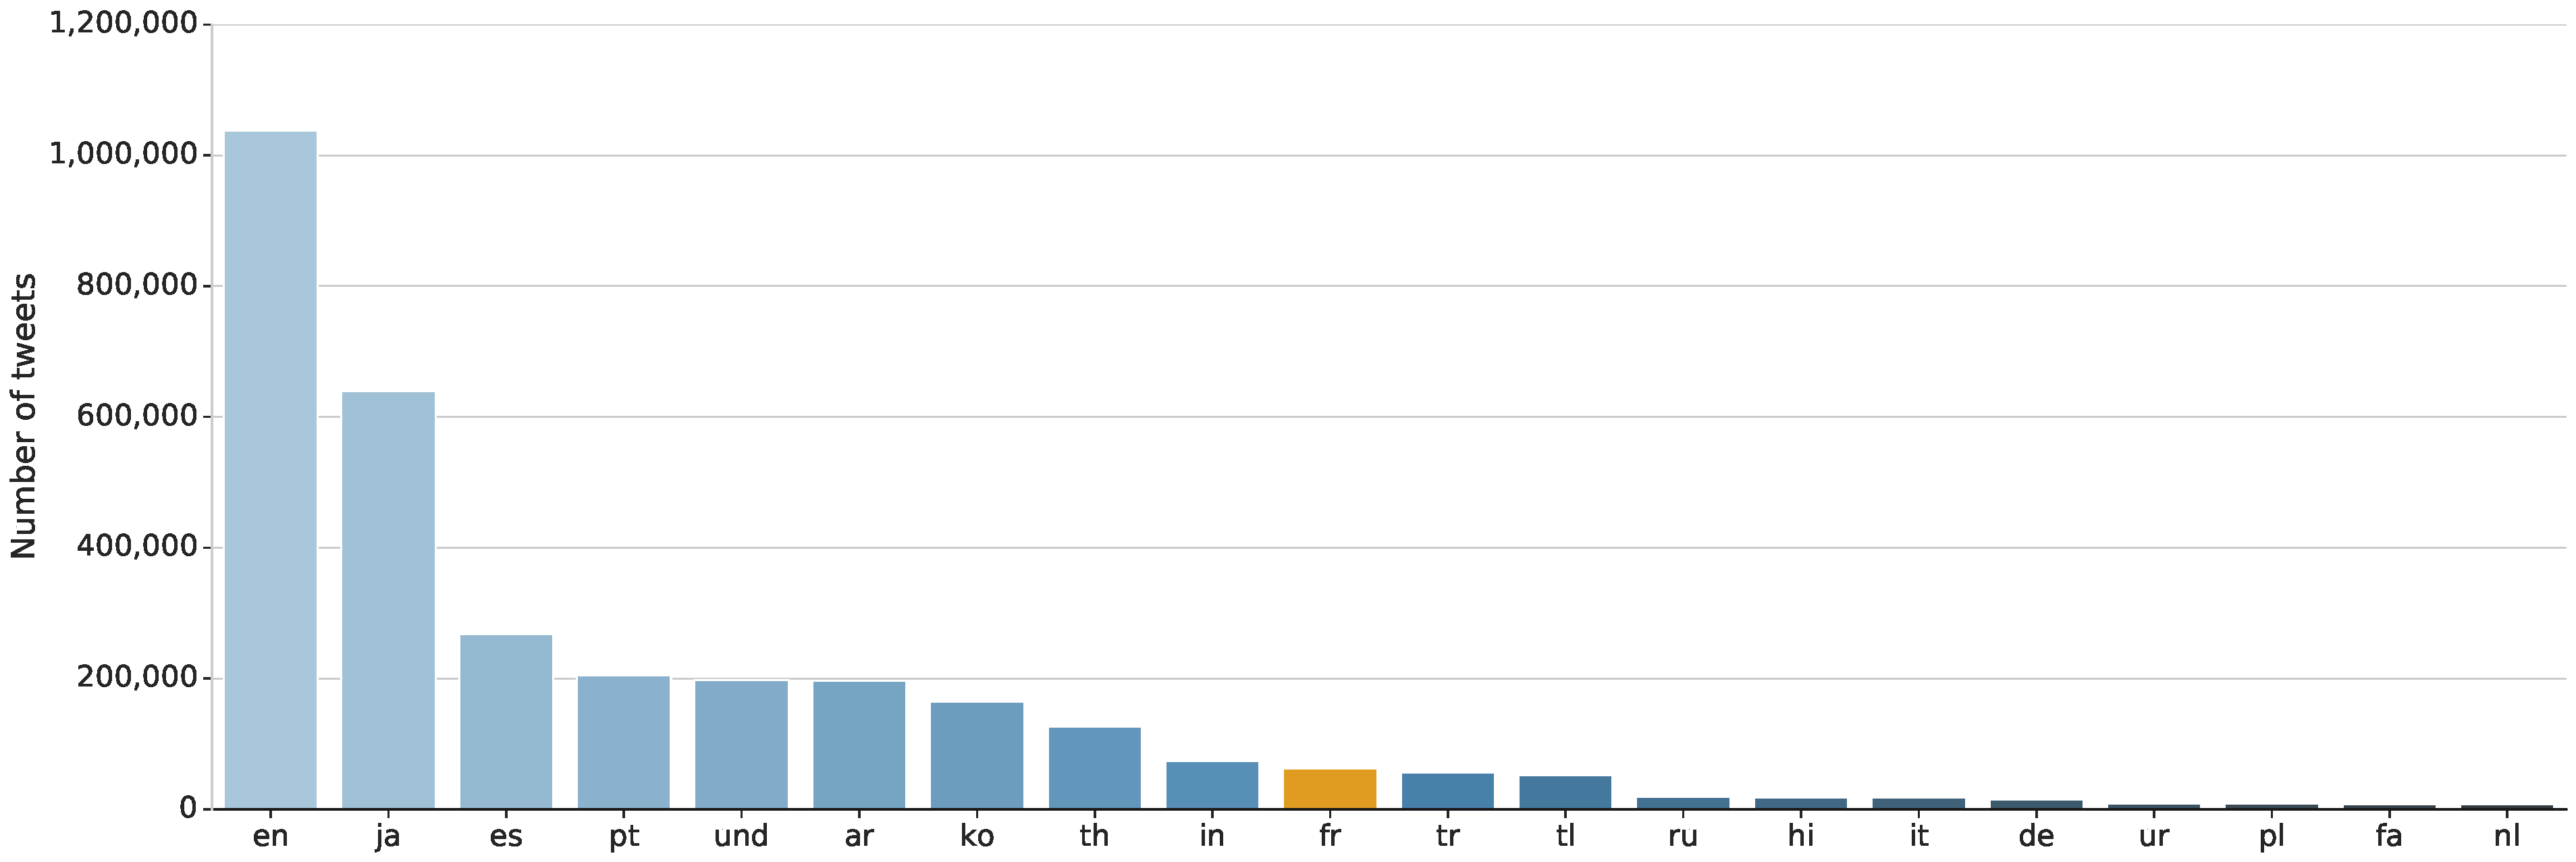
\includegraphics[width=1\textwidth]{figures/HistogramLanguages.pdf}
\end{center}
{\scriptsize \textbf{Notes:} This figure plots the average number of tweets collected  per day using the Sample API in the 20 most frequent languages on Twitter. The language metadata is provided by Twitter. "und" stands for "undefined" language.}
\caption{Average number of tweets in each language collected using the Sample API during one day}
\label{Figure:HistogramLanguages}
\end{figure}
%%%%%%%%%%%%%%%%%%%%%%%%


\paragraph{Filter API:}

the Filter API\footnote{\url{https://developer.twitter.com/en/docs/tweets/filter-realtime/api-reference/post-statuses-filter.html}} continuously provides tweets corresponding to the input parameters (keywords, account identifiers, geographical area). The language of the returned tweets can be selected. Again, the API provides only about 1\% of the total flow. However, this is sometimes enough to collect all the tweets containing a relatively little used keyword, and this is naturally enough to collect all the tweets from a given account. For a quite little represented language such as French, this API could theoretically provide us up to 55\% ($\frac{1\%}{1.8\%} = 55\%$) of the tweets emitted in French. Given this observation, we worked at identifying the keywords that maximize the number of returned French tweets.


\citet{joseph_two_2014} compare five samples collected through the Filter API with the same input keywords at the same time, using five different connection tokens\footnote{To use the Twitter API, a connection token is required. Twitter limits the access to its data by generating only one connection token per Twitter account.}: they find that two connections to the Filter API at the same time with the same keywords as inputs are ``nearly identical". It is hence not useful to try to get more tweets using a second access token with the same keywords. However, spreading different keywords over several API connections should return a higher number of tweets.

			\subsection{Proposed collection strategy \label{Subsec: collection strategy}}

Given the constraints of the APIs, we decided to collect tweets by using the random stream proposed by the Sample API, but to increase the volume of collected data by using the Filter API as well, with ``neutral" terms as keywords parameters, and ``French" as language parameter.  In order to further increase the volume, we decided to use multiple tokens to connect to the Filter API. 



The choice of the keywords parameters was done to optimize two metrics: the number of collected tweets, and their representativity of the real Twitter activity. The selected terms had thus to be the most frequently written on Twitter, and we had to use different terms (and terms that do not co-occur in the same tweets) as parameters for each connection. This way, the multiple connections would return sets of tweets with little intersection, and thus a greater total volume.


%%%%%%%%%%%%%%%%%%%%%%%%
\begin{figure}
\makebox[\textwidth][c]{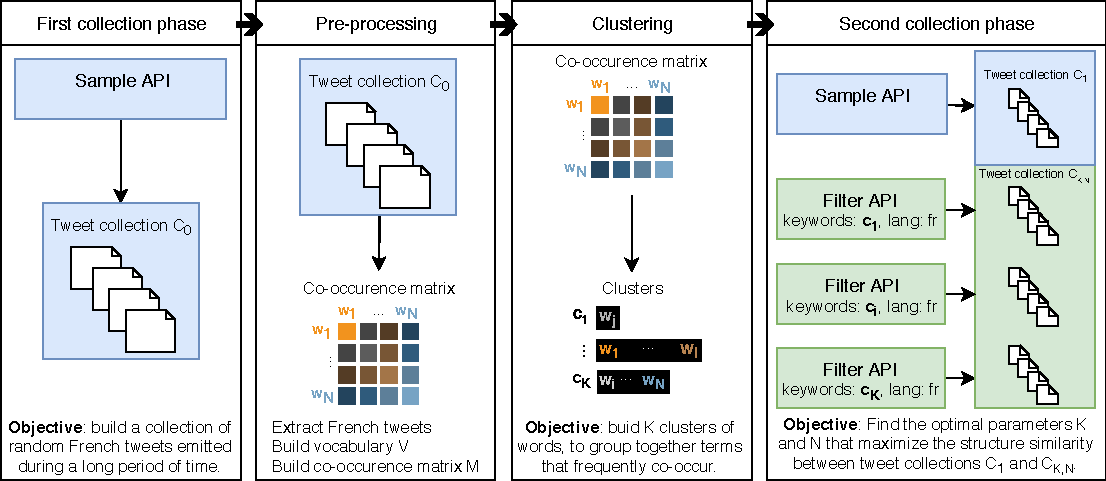
\includegraphics[width=1\textwidth]{figures/ExperimentalSetup.pdf}}
\caption{Diagram of our experimental setup to select the best tweet collection method}
\label{Figure:ExperimentalSetup}
\end{figure}
%%%%%%%%%%%%%%%%%%%%%%%%

The precise strategy was the following (it is schematized in figure \ref{Figure:ExperimentalSetup}): given a set of tweets $C_{0}=\{t_{1},\ldots, t_{k}\}$  collected using the Sample API during a time-interval $I = [d_{t,start}, d_{t,end}]$ we select tweets in French, creating a subset $C_{0 French}$ and extract from them a vocabulary $V = \{w_j, \forall j\in[1, \ldots,M]\}$ of all unique words appearing in $C_{0 French}$. We extract a subset of the $N$ words of $V$ having the highest document-frequency. We build a co-occurrence matrix $\mathcal{M} = (m_{i,j}) \in \mathbb{N}^{N\times N}$ where $(m_{i,j})$ is the number of times $w_i$ and $w_j$ co-occur in the same tweet of $C_{0 French}$. Using spectral clustering with $\mathcal{M}$ as adjacency matrix, we extract  $K$ clusters of terms. The $K$ obtained clusters of words are then used as parameters of $K$ different connections to the Filter API. By doing so, we aim at separating terms that are not frequently used together and thus to collect sets of tweets with the smallest possible intersection.


Section \ref{SubSec: evaluation_of_collection} presents the method used to evaluate the similarity between $C_{K,N}$ the set of tweets collected using $N$ keywords spread on $K$ Filter API connections, and $C_1 French$ the set of French tweets collected with the Sample API during the same period as $C_{K,N}$.

			\subsection{Experimental setup}

In practice, we collected our corpus $C_0$ of sample tweets between $d_{t,start} $ = 2018/01/15 and $d_{t,end}$ = 2018/02/15. The text of the collected tweets was tokenized on white spaces and on punctuation characters (``qu'il" was considered as two words, ``qu" and ``il"). The resulting vocabulary $V$ was lowercased and accents were removed, since we noticed that accents and capital letters are not taken into account by the Twitter API. For example, it returns tweets containing both ``à" and ``a" if the parameter ``a" is given as input. No other pre-processing such as stemming was applied (the vocabulary contains both ``mdr" and ``mdrrr"\footnote{French abbreviations similar to ``lol" and ``loool". ``mdr" stands for ``mort de rire", literally "laughing to death".}, for example), since the objective here is not to query the API with semantically different terms, but with the most frequently used terms.


 We ran tests with $N \in \{50, 100, 200\}$ and $K \in \{2,3\}$. This choice is motivated by our storage and CPU capacity. The clusters of terms for the different $N$ and $K$ values are presented in appendix \ref{Appendix: Clusters}. The resulting clusters are imbalanced in size: some contain only a few words, others contain all remaining terms. In order to control the effect of imbalanced clusters, we also tested to distribute terms randomly in clusters of size $\frac{N}{K}$. The samples collected using random clustering are denoted $R_{K,N}$. We ran each test for a period of two weeks, during which we also collected tweets from the Sample API and extracted tweets in French. This last set of tweets is denoted $C_{1 French}$.
			
			\subsection{Evaluation of the collection strategy \label{SubSec: evaluation_of_collection}}
			
%%%%%%%%%%%%%%%%%%%%%%%%%%%%
\begin{figure}
\begin{center}
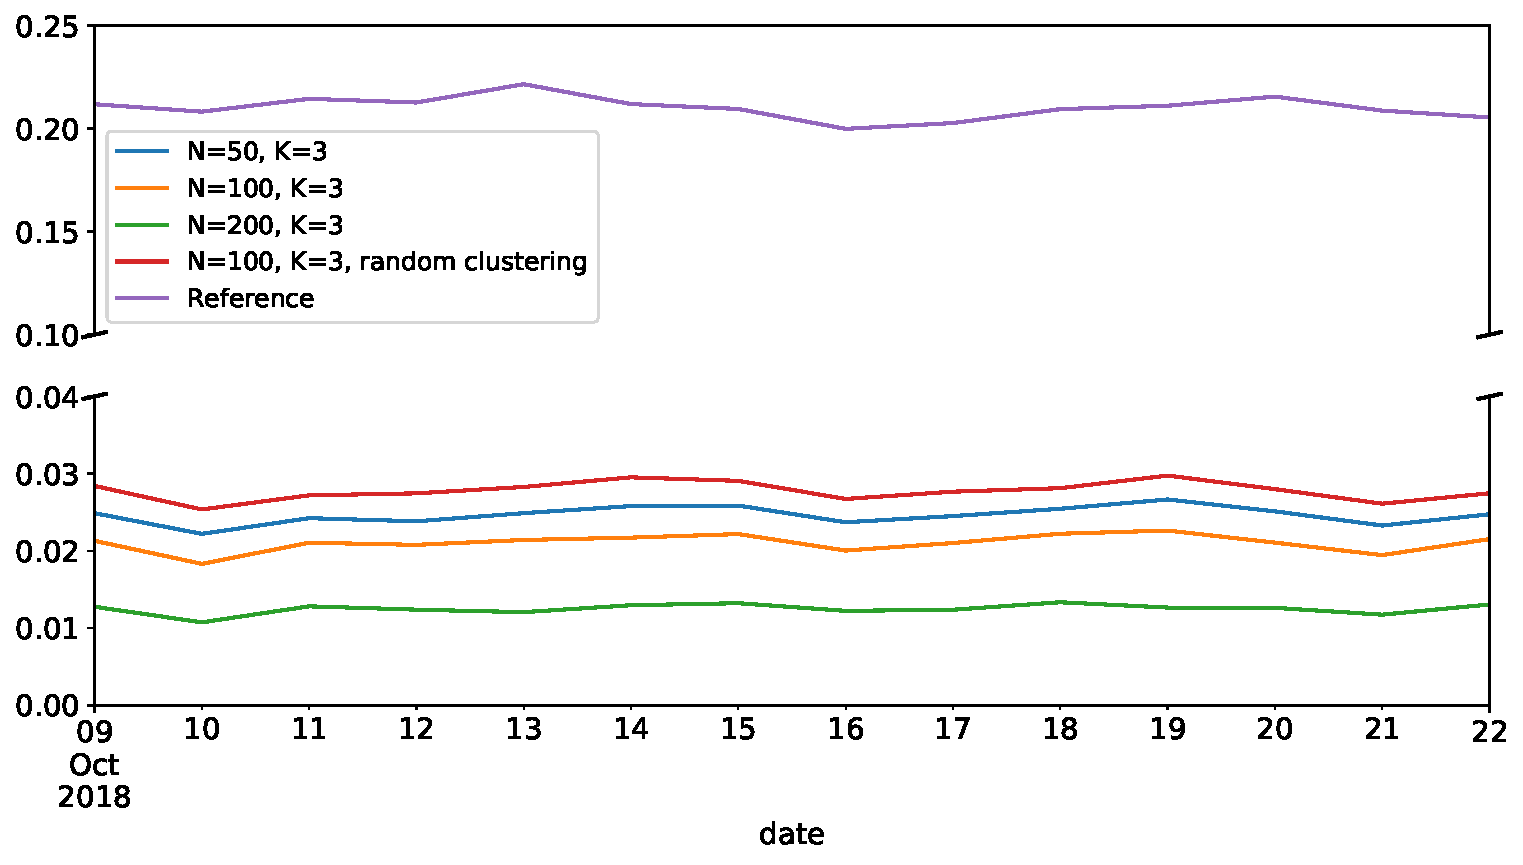
\includegraphics[scale=.5]{figures/KL_K=3.pdf}
\end{center}
{\scriptsize \textbf{Notes:} This figure plots the daily evolution of the KL-divergence between the word distribution in collection $C_1 French$ and the distribution obtained using 4 collection methods. The ``Reference" is obtained by splitting the collection $C_1 French$ in two sets and computing the KL-divergence between them. A KL-divergence of 0 indicates a perfect similarity between 2 distributions.}
\caption{Daily evolution of the divergence between collection $C_1 French$ and the collections $C_{K,N}$ with $K = 3$}
\label{Figure:KL_K=3}
\end{figure}
%%%%%%%%%%%%%%%%%%%%%%%%%%%%

We compared the sets $C_{K,N}$ and $R_{K,N}$ collected with each collection method with the set $C_{1 French}$ collected with the Sample API during the same time interval to assess the representativity of each test dataset. This approach is comforted by the study of \citet{morstatter_when_2014}, who have had access to the entire stream of tweets and compared it with the Sample API. They find that the tweets from the Twitter Sample API are ``a representative sample of the true activity on Twitter".  


Several comparison methods can be used in order to assess the similarity between two collections of texts. A first approach consists in considering the number of times each word is used in each collection as a probability distribution, and to measure the difference between those distributions. We used Kullback-Leibler divergence \citep{kullback_information_1997} as comparison metric. For two discrete probability distributions $P$ and $Q$ defined on the same probability space $\chi$ the Kullback-Leibler divergence is defined as
\begin{align}
\label{eq:KL}
KL(Q\|P) =  \sum_{x\in \chi}Q(x)\log{(\frac{Q(x)}{P(x)})}.
\end{align}
This measure is not symmetric, since it is meant to measure the difference between a probability distribution $P$ to a reference distribution $Q$, which is precisely what we have to evaluate, $Q$ being the distribution of words in $C_{1, French}$. For each $(N,K) \in  \{50, 100, 200\} \times \{2,3\}$, we computed the KL-divergence between the word distribution in $C_{K,N}$ and in $C_{1 French}$ for the same collection period. In order to have a reference of what level of divergence can be accepted, we also split the corpus $C_{1 French}$ in two sets (depending on whether the tweets had an even or odd id) and computed the KL-divergence between those sets. Figure \ref{Figure:KL_K=3} presents the results for $K=3$. Overall, we found that the collection $C_{3,200}$ was the most similar to $C_{1 French}$ using KL-divergence as comparison metric.


%This first way of evaluating the collection methods considers only the text of the tweets, without taking their structure into account: a tweet has an author, it is retweeted or not, it contains hashtags, urls, etc. In order to take the tweet samples' structure into account, we use  Student's t-tests to determine whether there is a significant mean difference between the two collections along several variables : 
%\begin{itemize}
%\item number of characters per tweet
%\item share of retweets (i.e. proportion of collected tweets that are actually retweets)
%\item share of quotes (i.e. proportion of collected tweets that quote another tweet)
%\item share of replies (i.e. proportion of collected tweets that reply to another tweet), 
%\item number of URLs per tweet
%\item number of hashtags per tweet
%\item share of ``verified users" (i.e. proportion of collected tweets from a user whose identity has been verified by Twitter)
%\item number of ``followers" of the tweet's author (i.e. accounts that subscribed to receive the tweets of this author)
%\item number of ``friends" of the tweet's author (i.e. the accounts to which the author subscribed)
%\item number of public ``lists" that the tweet's author is member of (any twitter account can create a public list of accounts, for example ``list of famous pianists")
%\end{itemize}

%%%%%%%%%%%%%%%%%%%%%%%%%%%%
%\begin{table}
%\begin{center}
%\makebox[\textwidth][c]{{
\def\sym#1{\ifmmode^{#1}\else\(^{#1}\)\fi}
\begin{tabular}{l*{1}{>{\bfseries}ccccc}}
\hline\hline
                    &\multicolumn{5}{c}{}                           \\
                    &$C_{1French}$&$C_{3,200} \cup C_{1French}$&$C_{3,100} \cup C_{1French}$&$C_{3,50} \cup C_{1French}$&$R_{3,100} \cup C_{1French}$\\
\hline
Number of characters&  116&    7\sym{***}&   8\sym{***}&   10\sym{***}&    9\sym{***}\\
                    &     &           (0)&          (0)&           (0)&           (0)\\
Share of retweets   & 0.61& 0.02\sym{***}&0.02\sym{***}& 0.02\sym{***}& 0.02\sym{***}\\
                    &     &        (0.00)&       (0.00)&        (0.00)&        (0.00)\\
Share of quotes     & 0.18& 0.01\sym{***}&0.01\sym{***}& 0.02\sym{***}& 0.01\sym{***}\\
                    &     &        (0.00)&       (0.00)&        (0.00)&        (0.00)\\
Share of replies    & 0.19&-0.02\sym{***}&-0.01\sym{***}&-0.01\sym{***}&-0.02\sym{***}\\
                    &     &        (0.00)&       (0.00)&        (0.00)&        (0.00)\\
Number of URLs      & 0.24& 0.01\sym{***}&0.01\sym{***}& 0.01\sym{***}&  0.01\sym{***}\\
                    &     &        (0.00)&       (0.00)&        (0.00)&        (0.00)\\
Number of hashtags  & 0.24&-0.01\sym{***}&-0.05\sym{***}&-0.06\sym{***}&-0.05\sym{***}\\
                    &     &        (0.00)&       (0.00)&        (0.00)&        (0.00)\\
Share of verified users&0.01&-0.00\sym{*}&        -0.00& -0.00\sym{**}& 0.00\sym{***}\\
                    &     &        (0.00)&       (0.00)&        (0.00)&        (0.00)\\
Number of followers &3,073&           -68&          -72&   -165\sym{*}&            59\\
                    &     &          (74)&         (74)&          (72)&          (76)\\
Number of friends   &  692&     -9\sym{*}& -34\sym{***}&  -44\sym{***}&  -30\sym{***}\\
                    &     &          (4) &          (4)&           (3)&           (4)\\
Number of lists     &   38&             0&            0&            -0&    2\sym{***}\\
                    &     &           (0)&          (0)&           (0)&           (0)\\
\hline
Observations        &875,630&  63,296,610&   59,118,730&    64,272,167&    55,405,602\\
\hline\hline
\end{tabular}
}
}
%\end{center} 
%	\scriptsize * $p < 0.1$, ** $p < 0.05$, *** $p < 0.001$. Standard errors in parentheses.\\
%	\scriptsize \textbf{Notes:} The table presents summary statistics for the collected samples using Student's t-tests for the equality of means. The first column (in bold) presents the mean of the tested variables in the reference sample $C_{1French}$. The next columns show the mean differences between that reference sample and the samples collected with each method.
%	\caption{Mean difference between each collection $C_{K,N}$, $K = 3$ and collection $C_{1French}$ }. 
%	\label{Tab:ttest_sample_c3200}
%\end{table}
%%%%%%%%%%%%%%%%%%%%%%%%%%%%

%%%%%%%%%%%%%%%%%%%%%%%%
\begin{figure}
\begin{center}
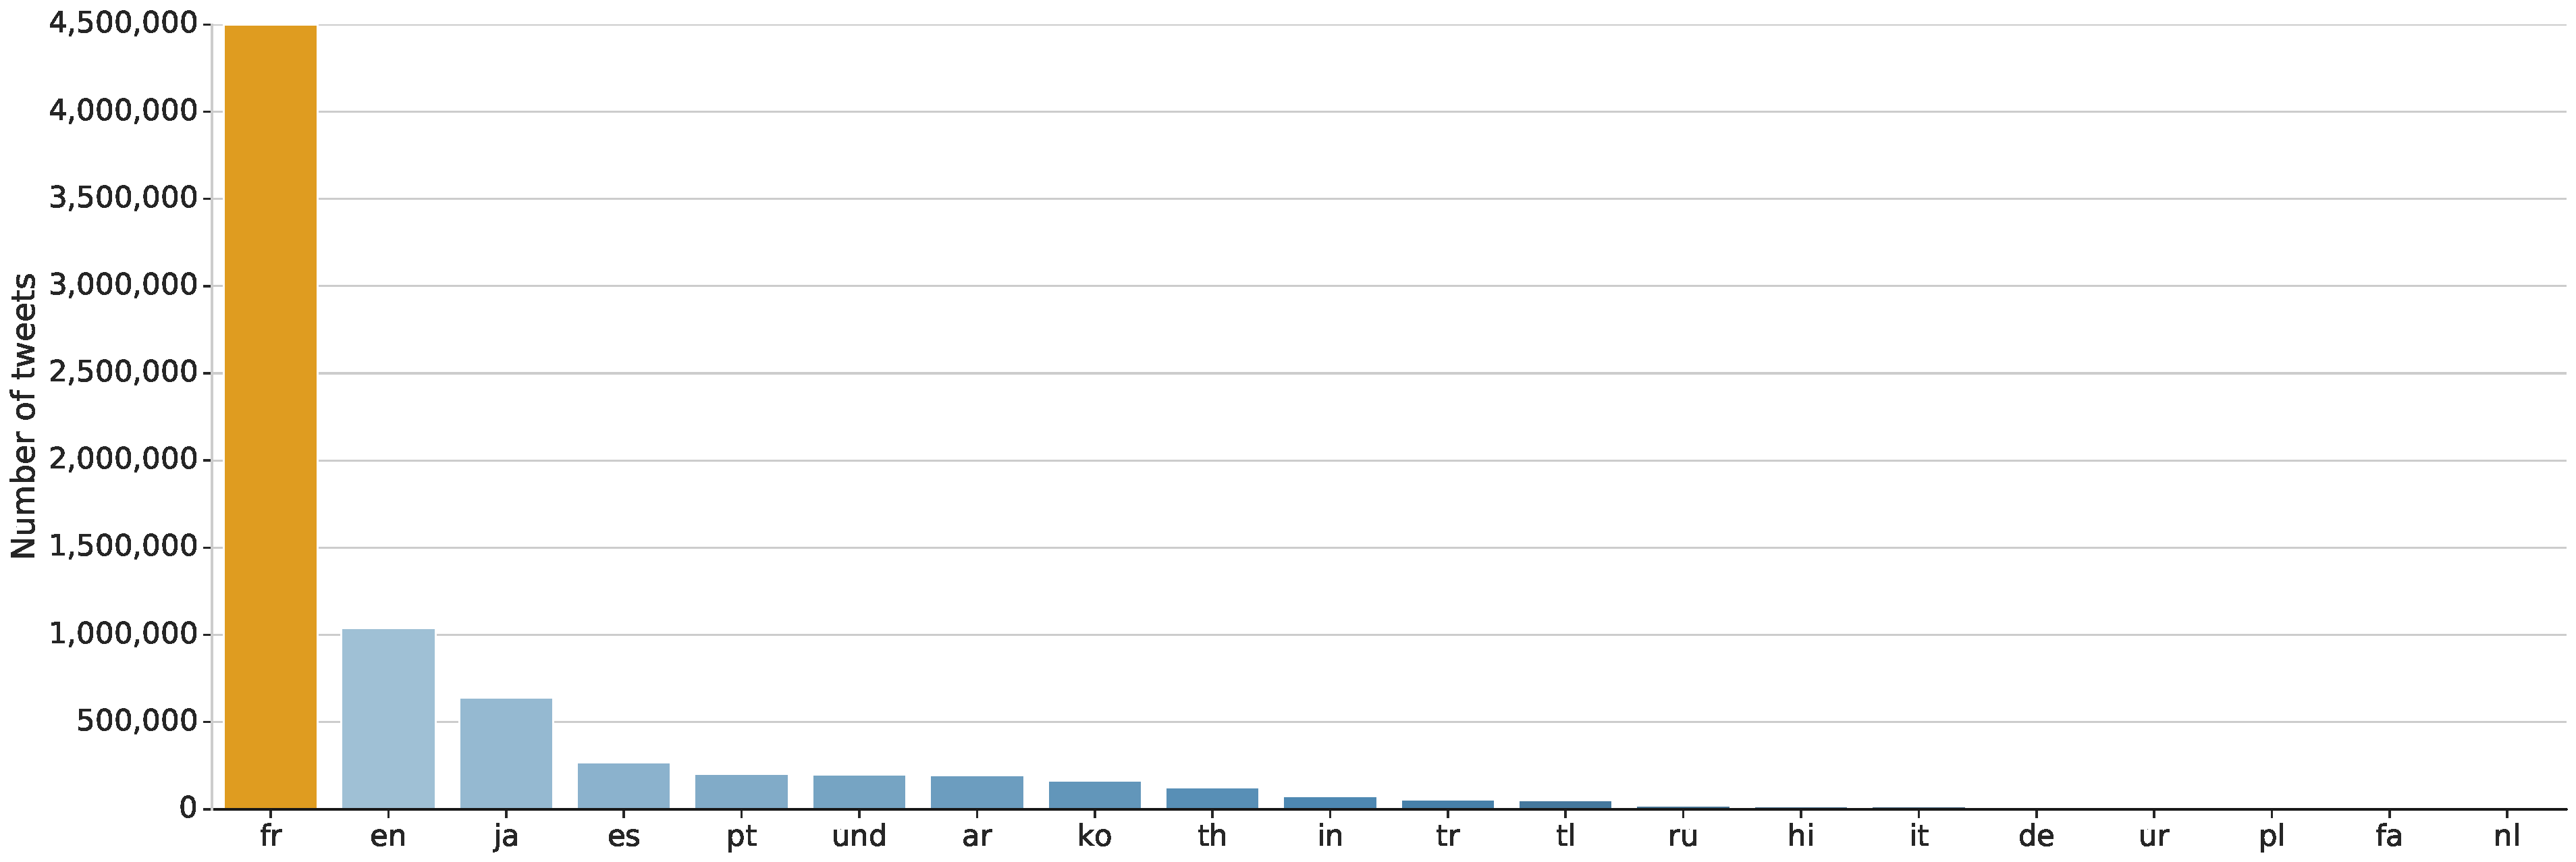
\includegraphics[width=1\textwidth]{figures/HistogramLanguagesFilter.pdf}
\end{center}
\scriptsize \textbf{Notes:} This figure plots the average number of tweets collected per day using our best collection method in the 20 most frequent languages on Twitter. The language metadata is provided by Twitter. "und" stands for "undefined" language.

\caption{Average number of tweets per day in each language collected using the Sample API combined to our best collection method}
\label{Figure:HistogramLanguagesFilter}
\end{figure}
%%%%%%%%%%%%%%%%%%%%%%%%

%Table \ref{Tab:ttest_sample_c3200} summarize Student's t-tests for the samples collected with 3 clusters (K=3) compared to the random sample $C_{1French}$. All collection methods have a statistically significant mean difference to the random sample on all tested variables (except the number of followers, where there is no significant mean difference between the collection methods). However, the difference is small, particularly for the best collection method  ($C_{3,200} \cup C_{1French}$): +0.01 for the number of URLs and -0.01 for the number of hashtags) which indicates a very similar structure of the conversations.  The number of characters tends to be significantly higher in our collection methods than in the random sample (+7 characters for $C_{3,200} \cup C_{1French}$), which can be explained by the fact that our collection methods return tweets containing the keywords given as input parameters, excluding \textit{de facto} all tweets that contain no word. 


We decided to keep $C_{3,200} \cup C_{1French}$ as main collection method, since its similarity to the random sample was the highest. Figure \ref{Figure:HistogramLanguagesFilter} illustrates the new distribution of language using that method.

\subsection{Evaluate the share of collected tweets}

The tweet collection tool has been running from June 2018 to the present day, allowing us to store around 3 billion tweets. This long collection period allowed us to compare our corpus with other French tweet corpora collected during that time. Two teams were kind enough to give us access to part of their data: the French Internet legal deposit at the INA, and the Médialab at Sciences Po Paris. We also used metrics from Twitter (the number of tweets per user) to estimate the percentage of tweets that we collect, and conversely, the number of tweets we miss.

\subsubsection{Corpus provided by the French Internet legal deposit (DLWeb)}
%%%%%%%%%%%%%%%%%%%%%%%%
\begin{figure}
\begin{center}
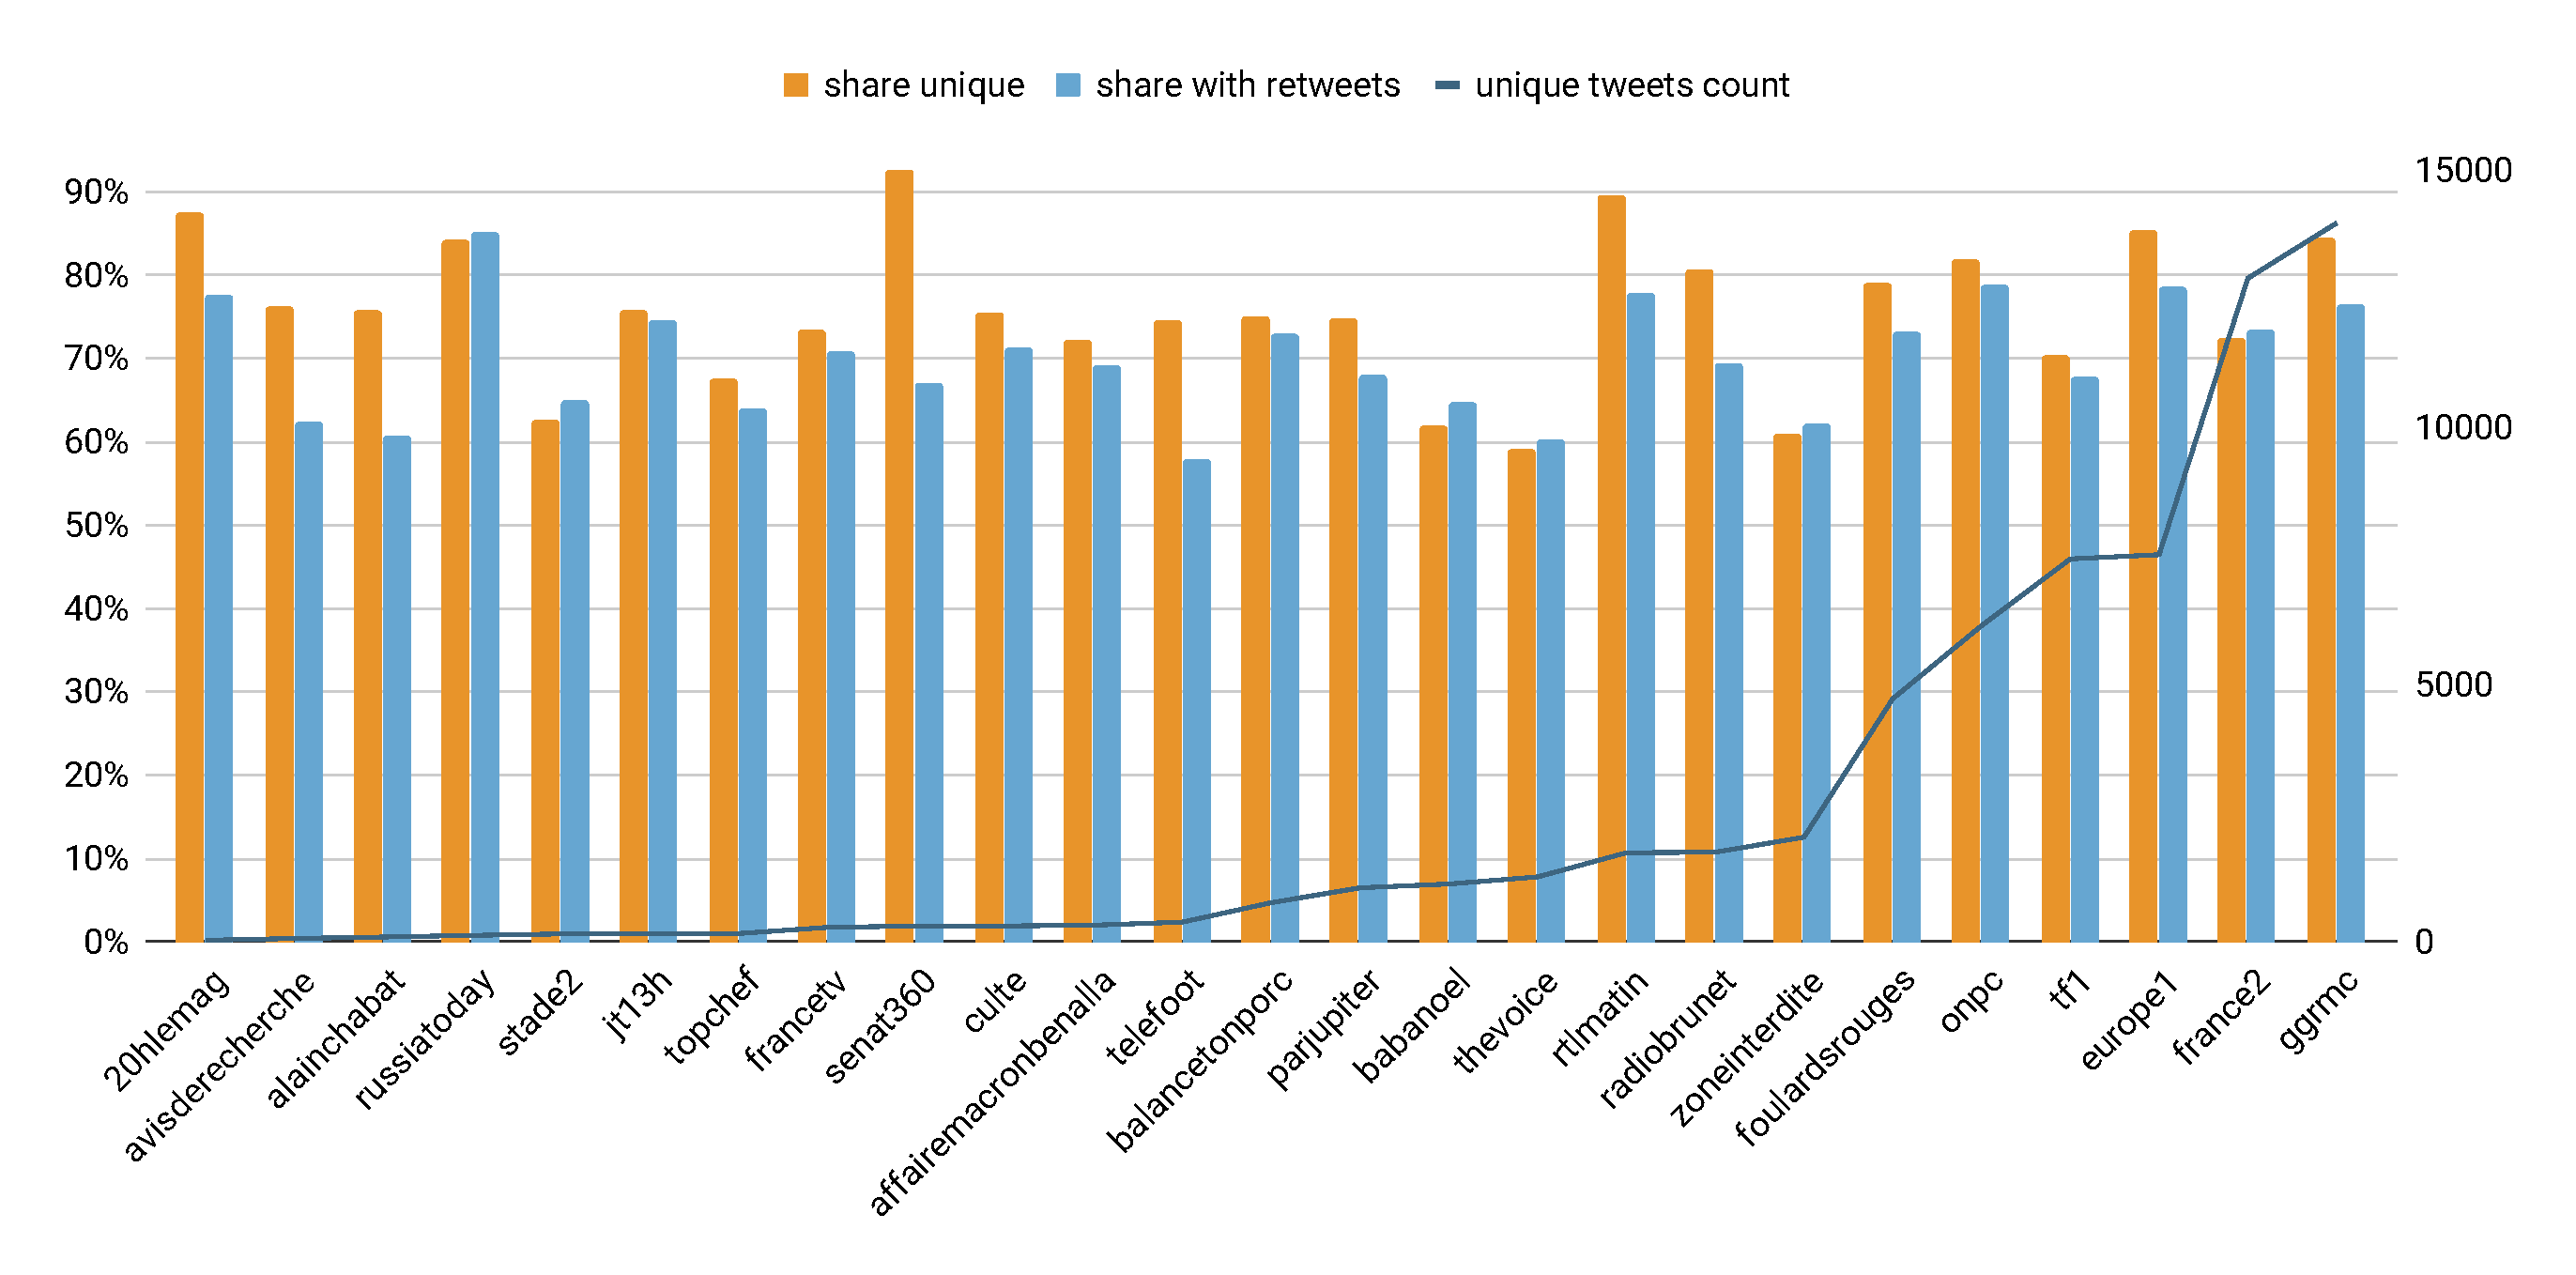
\includegraphics[width=1\textwidth]{figures/ShareinCommonWithDL.pdf}
\end{center}
\scriptsize \textbf{Notes:} This figure plots the share of tweets from the DLWeb that we were also able to capture using our collection method. Blue columns represent the ratio for all tweets, yellow columns represent the ratio for original tweets (\textit{i.e.} retweets excluded). The grey line shows the number of original tweets (\textit{i.e.} retweets excluded) captured by the DLWeb for each hashtag. Tweets were collected from December 1st to December 31st, 2018.

\caption{Share of DLWeb tweets captured using our collection method for a set of 25 hashtags}
\label{Figure:HistogramHashtagsDLWeb}
\end{figure}
%%%%%%%%%%%%%%%%%%%%%%%%

The French Internet legal deposit department at the INA is in charge of archiving French websites related to audiovisual media (television, radio, web TVs). As part of this mission, the team collects tweets concerning audiovisual media and therefore regularly updates a manually curated list of hashtags and Twitter accounts to be captured using the Filter API. The DLWeb team provided us with the tweets collected for 25 of these hashtags over the course of a month, and we counted how many of these tweets had been collected over the same period using our method. The results are presented in Figure \ref{Figure:HistogramHashtagsDLWeb}. In average, we collected 74\% of the tweets from the DLWeb, and 78\% if we exclude retweets. Original tweets are better captured than retweets by our collection method, because each retweet allows us to archive the original tweet to which it refers. Therefore, we only need to capture one of the retweets of a tweet to get the original tweet. Retweets, on the other hand, are not retweeted, so we lose any chance of catching them if they were not obtained at the time they were sent.

It should also be mentioned that the DLWeb does not guarantee to collect all tweets containing a given hashtag. Capturing on specific hashtags allows them to get a larger share of the tweets containing these hashtags than we do, but we also captured some tweets that they didn't collect. Overall, since Twitter does not communicate on this subject, it is difficult to evaluate precisely why the relative performance of the collection methods varies depending on the hashtag. The volume collected by the DLWeb may depend on the popularity of the hashtag, and the popularity of other collected hashtags during the same time period. 

In order to validate our collection method with a more stable comparison dataset, we computed the same metrics on a second corpus, presented in the next section.

\subsubsection{Corpus provided by the Médialab team}
We compared our collection with the corpus of tweets built by \citet{cardon2019unfolding}, that consists of
tweets containing URLs from a curated list of 420 French media sources. The Médialab team uses different API endpoints to search for tweets that contain one of the selected domain names, including the Filter API but also the Search API\footnote{\url{https://developer.twitter.com/en/docs/tweets/search/api-reference/get-search-tweets}} that returns tweets matching a query within the last 7 days. They gave us access to a part of their dataset, namely all tweets collected between December 1st and 31st 2018, amounting to 8.7 million tweets. Among these tweets, we only kept those in French, i.e. 7.3 million tweets. Our sample contains 70\% of these tweets in French, and 74\% if we exclude retweets. Figure \ref{Figure:HistogramUrlsMedialab} shows the percentage of collected tweets for the most important domain names in terms of number of original tweets (\textit{i.e.} retweets excluded) in the Médialab dataset.

%%%%%%%%%%%%%%%%%%%%%%%%
\begin{figure}
\begin{center}
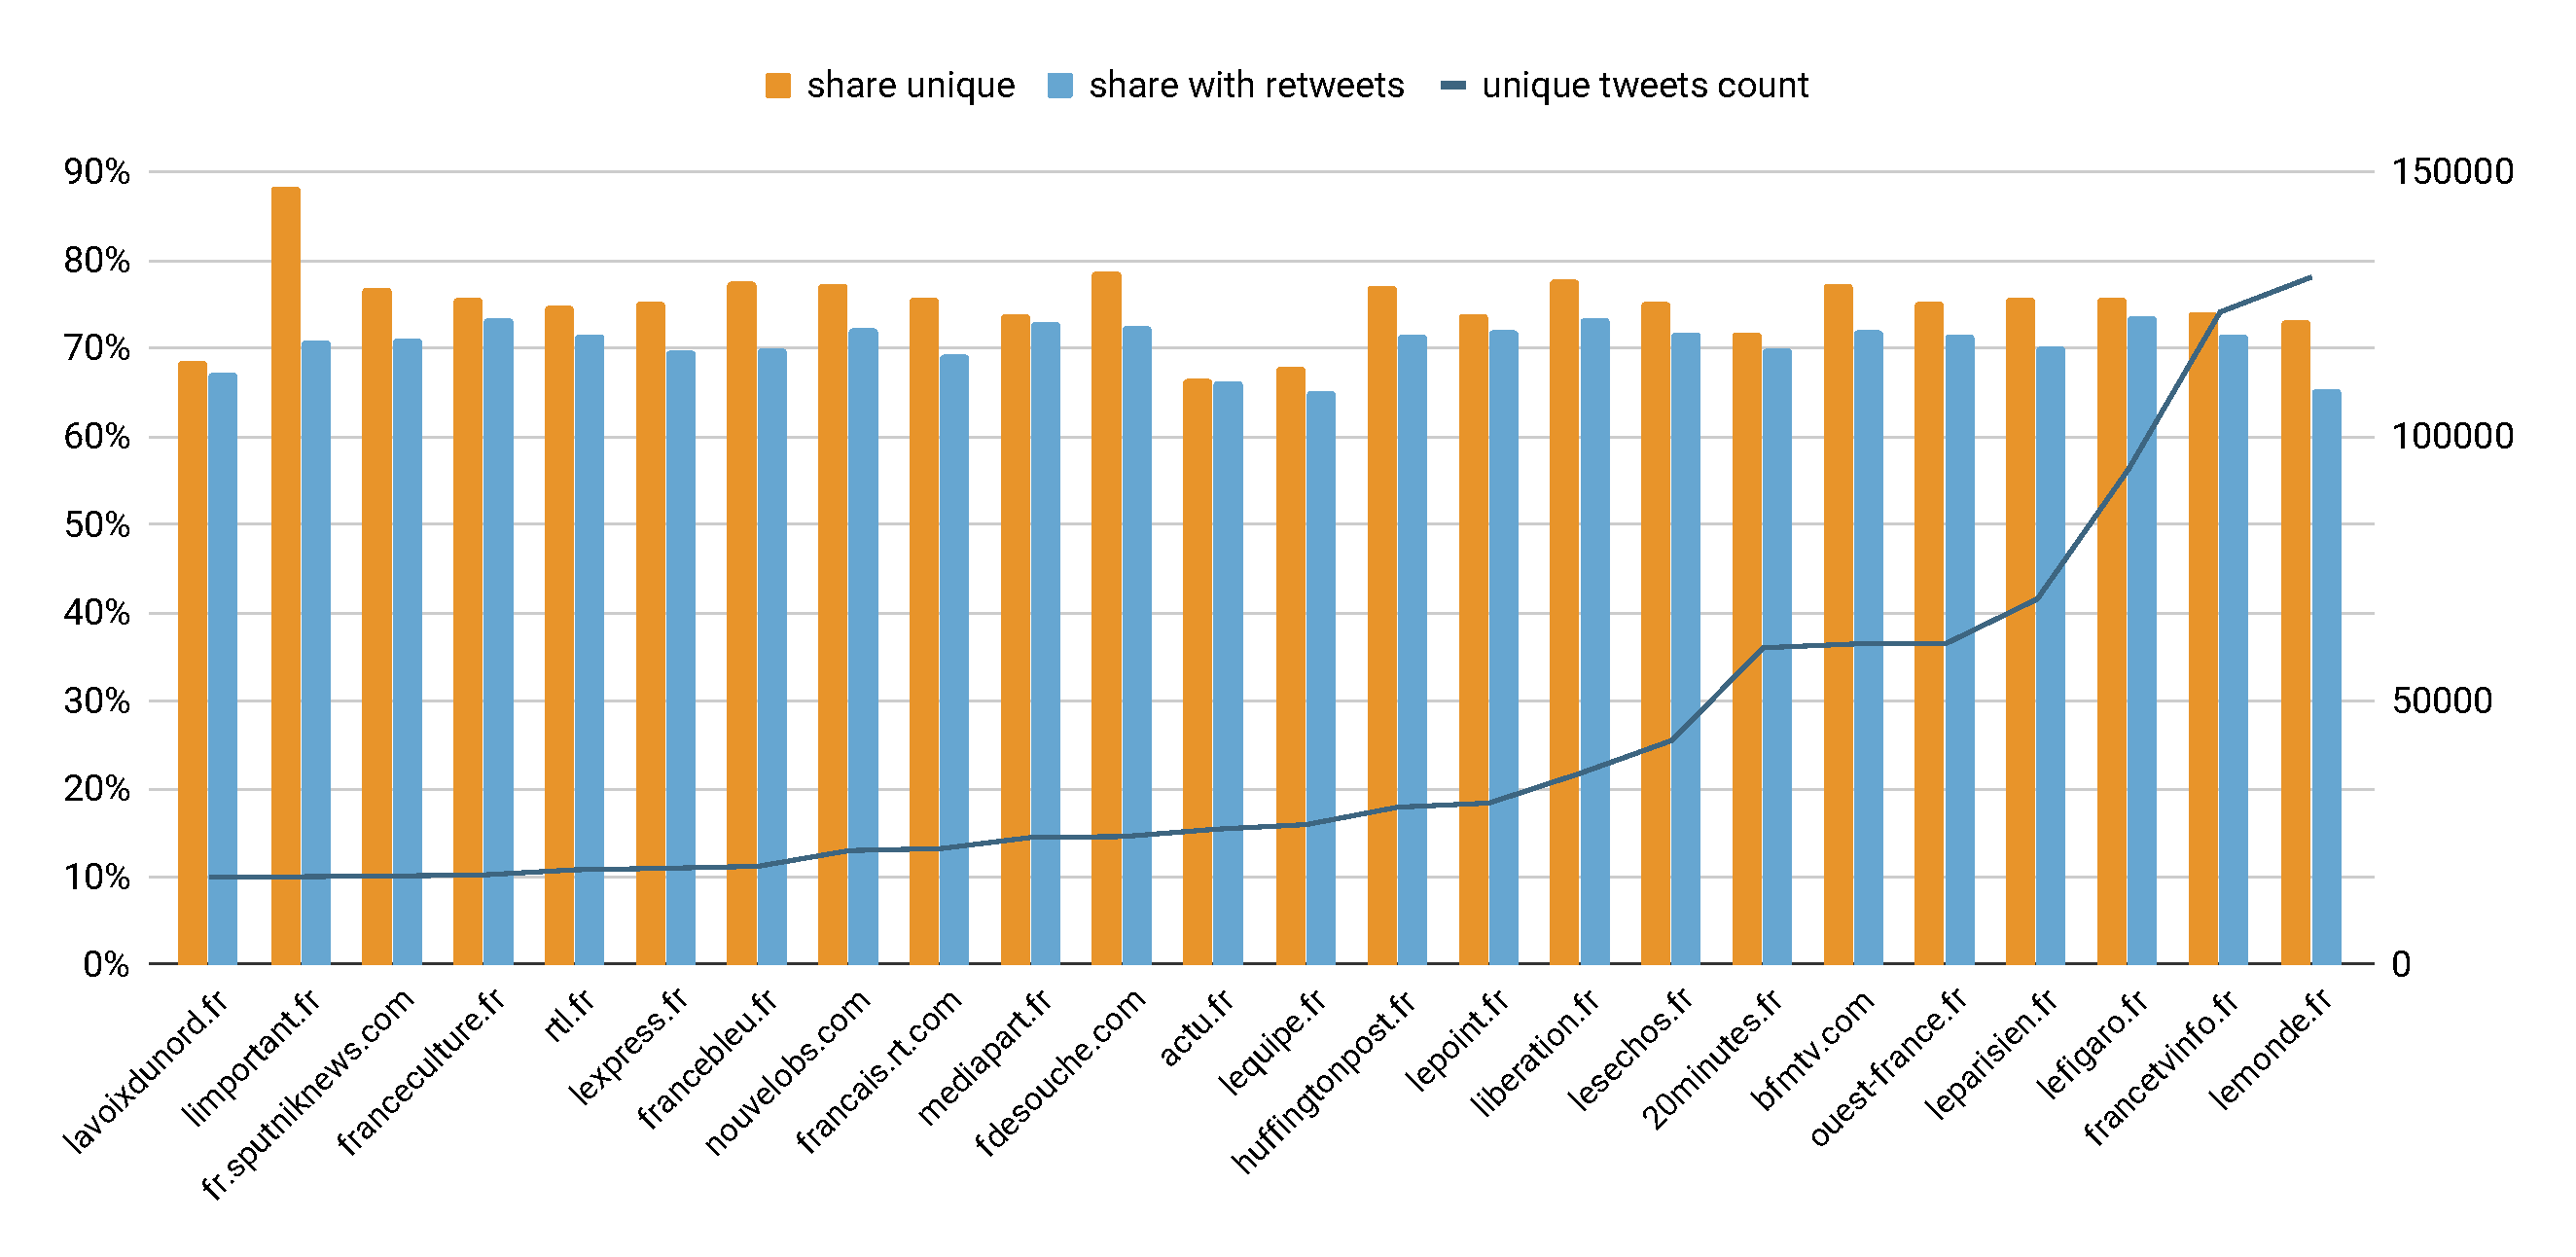
\includegraphics[width=1\textwidth]{figures/ShareInCommonWithMedialab.pdf}
\end{center}
\scriptsize \textbf{Notes:} This figure plots the share of tweets from the Médialab that we were also able to capture using our collection method for the 25 first domain names in terms of original tweets in their dataset. Blue columns represent the ratio for all tweets, yellow columns represent the ratio for original tweets (\textit{i.e.} retweets excluded). The grey line shows the number of original tweets (\textit{i.e.} retweets excluded) captured by the Médialab for each domain. Tweets were collected from December 1st to December 31st, 2018.

\caption{Share of tweets from the Médialab also captured using our collection method for 25 domain names}
\label{Figure:HistogramUrlsMedialab}
\end{figure}
%%%%%%%%%%%%%%%%%%%%%%%%

\subsubsection{Evaluate the number tweets per user}

A third method can be used to compare our sample with the real number of tweets in French emitted on Twitter. It is based on the total number of tweets sent by a user since the account creation, a metadata that is provided by Twitter for every new tweet. With this metric, we can get an estimate of the total number of tweets emitted by a given user between two of its tweets. We can then compare this value with the number of tweets actually collected for that user.

In practice, we selected the tweets of all users that had written at least 3 tweets in 3 months (from July 1st to September 30th 2018), retweets included. In order to select users that write mostly in French (tweets written in other languages are not collected with our method), we used the OpenStreetMap API to locate users depending on what they indicate in the "location" field. We obtained 920,000 users localized in France that emitted 241 million tweets in three months, according to the "number of tweet" field. With our collection method, we captured 147 million tweets from these users, \textit{i.e.} 61\% of the real number of emitted tweet. We found the same percentage with the sample of users who geolocate their tweets in France (27,000 users). This method gives us a high estimate of the real number of emitted tweets in French, since some of these users probably write in other languages than French, even if they are located in France.

All three comparison methods have their flaws, however they produce close results. We can therefore conclude that we collect between 60\% and 75\% of all tweets in French sent on Twitter. We were therefore able to build our annotated dataset with the guarantee that our sample of tweets is representative. The next section presents the annotation procedure.

\section{Tweet annotation}

We built our event detection corpus based on tweets collected with our collection method from July 15 to August 6, 2018. During this period, we collected 38 million original tweets (retweets excluded). We annotated these tweets depending on their relation to  Twitter events and media events that took place in France at the time of the annotation.
	
	\subsection{Media events selection}
	To select media events, we decided to draw events randomly
from the hundreds of events described in French press every day. We drew press articles for every day from July 15 to August 6, 2018, for a total of 23 days. We did not want to use any automatic detection method to generate events from the collected tweets, since it may bias the results of our evaluation tests (detection methods similar to the one used to generate events in the test set may be advantaged). We did not either use Wikipedia to select important events (like it is the case in \citet{mcminn_building_2013} and \citet{petrovic_using_2012}), considering that ``an event detection system should also be able to detect newsworthy events at a smaller scale" \citep{hasan_survey_2018}. 


In practice, we drew 30 events a day, two thirds from the Agence France Presse (AFP), which is the third largest news agency in the world, and one third from a pool of major French  newspapers (\textit{Le Monde}, \textit{Le Figaro}, \textit{Les Échos}, \textit{Libération}, \textit{L'Humanité}, \textit{Médiapart}). This selection method has the advantage of giving ``big" events a higher chance of being selected, since they are covered by all news outlets, while also letting relatively ``small" events emerge. Duplicates, that is to say articles covering the same event, were manually removed. 30 events seemed to us to be the maximum number of events the annotators could process in one day. In reality they did not have time to annotate most of them, and only processed the beginning of the list each day.
Since new events were drawn every day, events that continued over several days were considered as separated events at the time of annotation. We then grouped together these daily events manually.

\subsection{Twitter events selection}
\label{Twitter events selection}
Since our final objective is to measure differences in the coverage of events by news media and by Twitter users, we did not want to miss important events in the Twitter sphere that would be little covered by traditional news media. We therefore monitored the trending terms on Twitter by detecting unusually frequent terms every day. 


We chose a metric called $JLH$, that is used by Elasticsearch\footnote{\url{https://www.elastic.co/guide/en/elasticsearch/reference/current/search-aggregations-bucket-significantterms-aggregation.html\#_jlh_score}}  to identify ``significant terms" in a subset of documents (\textit{foreground set}) compared to the rest of the collection (\textit{background set}). It simply compares for each term $t$ the frequency of appearance in the foreground set ($p_{fore}$) and in the background set ($p_{back}$). This metric is computed as:

$$
f(t,d) = \left\{
	\begin{array}{ll}
		(p_{fore}(t,d) - p_{back}(t))\frac{p_{fore}(t,d)}{p_{back}(t)} & if\, p_{fore}(t,d) - p_{back}(t) > 0\\
		0 & elsewhere
	\end{array}
\right.
$$
Where $p_{fore}(t,d) = \frac{tf(t,d)}{u_d}$  (the number of different users mentioning term $t$ on day $d$ divided by $u_d$ the total number of users tweeting on day $d$) and $p_{back}(t)  = \frac{tf(t)}{U}$ (the number of different users mentioning term $t$ in the total collection divided by $U$  the total number of users, measured by the number of different authors of tweets in our collection). We did not use a standard $\mbox{tf-idf}$ metric because it resulted poorly at identifying bursting terms for a given a day.


We computed the 20 terms having the best $JLH$ scoring every day and went on Twitter to discover the underlying events causing a burst of these terms. We were then able to group together terms related to the same event. For example the terms ``afcbom", ``bournemouth", ``bouom", ``afcbournemouth", all related to a soccer match between the Association Football Club Bournemouth (AFCB) and the Olympique de Marseille (OM), were grouped together. We then excluded events:
\begin{itemize}
\item that were artificially amplified using automatic tools. In particular, the Q\&A website Curious Cat was used to post the same questions (``Where do you see yourself in tens years from now?", ``What is your favorite movie?") to all Twitter users registered on Curious Cat. Many of them responded using the terms of the question (``My favorite movie is...") causing a burst in the frequency of those terms.
\item that had been already drawn from the media events selection process.
\end{itemize}

Once the media events and the Twitter events selected, the annotators' work could begin. In the following section, we explain the annotation procedure.
		\subsection{Annotation procedure}
		\subsubsection{User interface}
		
%%%%%%%%%%%%%%%%%%%%%%%%
\begin{figure}
\begin{center}
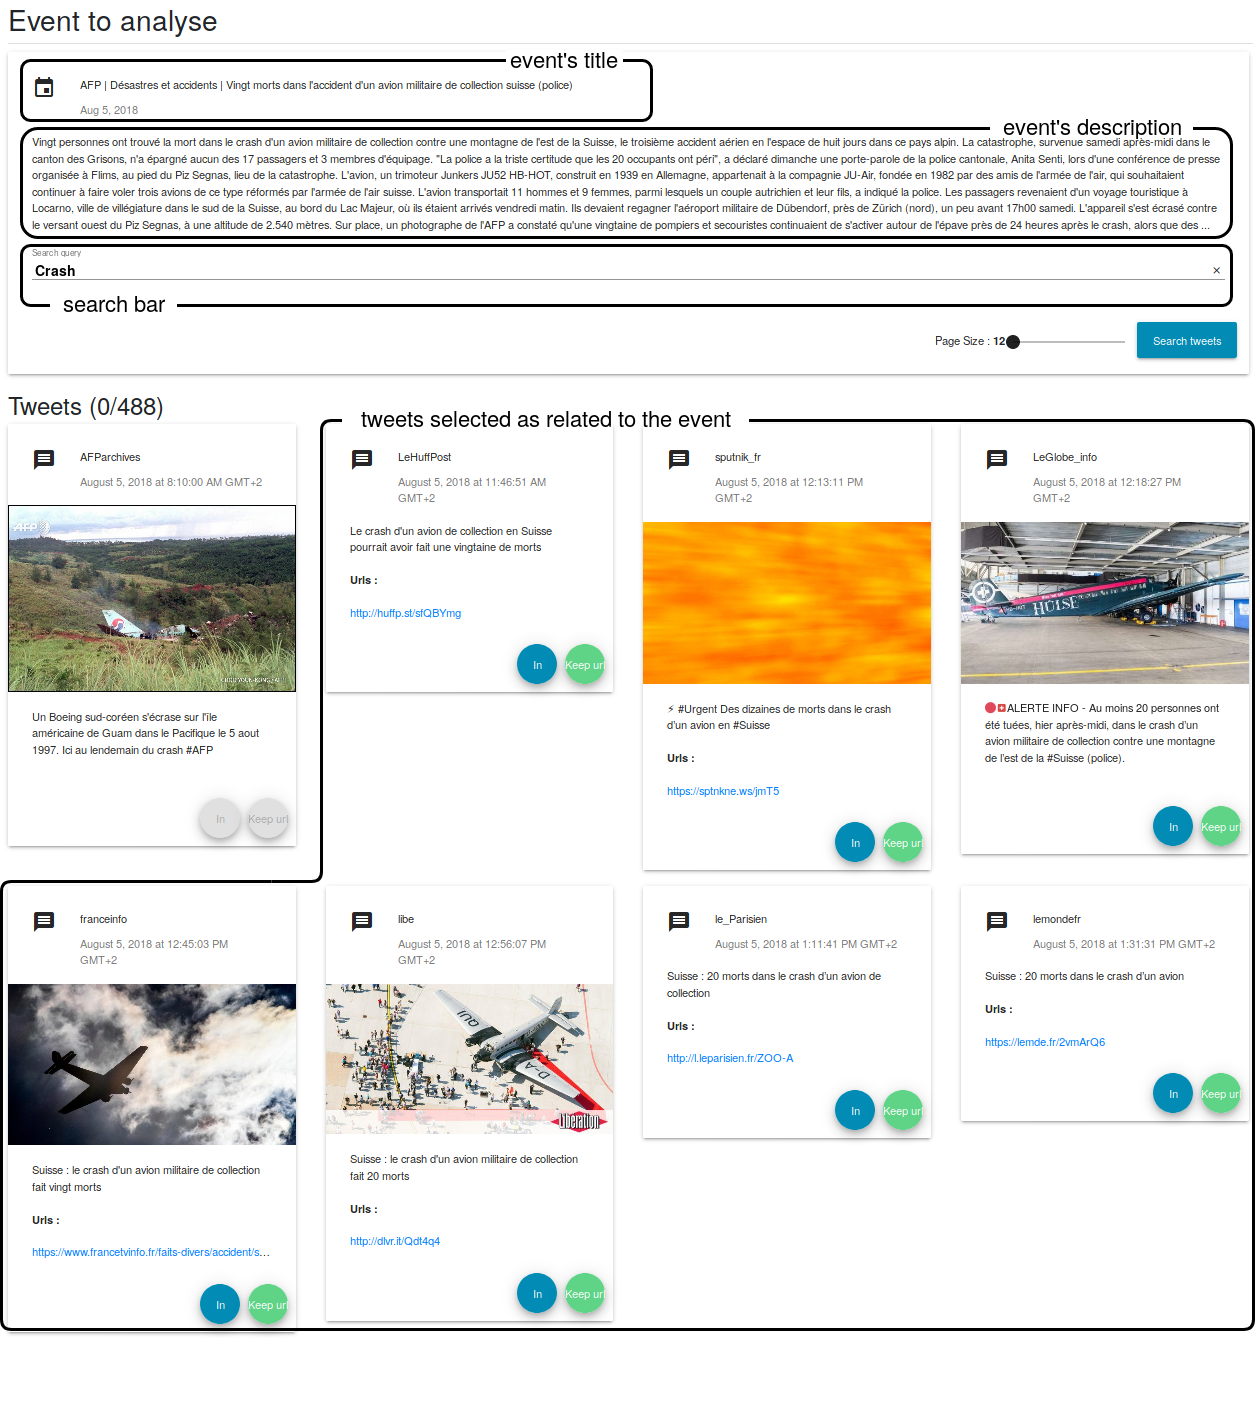
\includegraphics[width=1\textwidth]{figures/Crash_with_comments.png}
\end{center}

\caption{View of the annotation interface}
\label{Figure:Interface}
\end{figure}
%%%%%%%%%%%%%%%%%%%%%%%%
We developed a user interface (see Figure \ref{Figure:Interface}) presenting each event in the form of a title and a description text. For media events we used the title and the first paragraphs of the drawn corresponding press article. For Twitter events the title was constituted of the bursting terms detected with the $JLH$ scoring and the description was a tweet manually selected because it described the event clearly. Under the title and the description, a search bar was presented. The user could use that bar to enter keywords and find the collected tweets containing those exact keywords. Twelve tweets per page were displayed, starting with the most retweeted. The user could select or unselect the tweets he considered related to the event. If the tweet contained an URL, the user could click or unclick a button under the tweet to indicate if the linked page was related to the event as well. Once the user had read all twelve tweets and selected the ones related to the event, the user could submit its answers and access to the next twelve tweets. Displayed tweets were not pre-selected by our program depending on their content. We only excluded retweets since it would only have displayed the same tweet several times, and displayed tweets emitted on the day of the event. 


The interface also allowed to review tweets annotated by other users: once an annotator was finished with an event, she could access another page displaying the same event (same title, same description) and the tweets seen by other annotators in relation to the event. The user had to go through all these tweets and annotate them, without knowing if those tweets were marked as relevant or irrelevant to the event by the other users.

		\subsubsection{Annotation task}
	Three political science students were hired for a month to annotate the corpus. All three of them were Twitter users and had a good knowledge of media news. Every day they were presented the new list of events. They started on the 16th of July, 2018, to annotate events from the 15th of July. This first day of annotation was not included in the final dataset and served as a day of adaptation. Since the annotators did not work on Saturday or Sunday, every day between July 15th and August 15th could not be annotated. We made the choice to annotate on a continuous period of time, from the 16th of July to the 6th of August.


For every event, they were asked to search for related tweets on the user interface, using a large variety of keywords. It was insisted on the importance of named entities (persons, locations, organizations) and on the specificity of Twitter (one person can be referred to using her real name or her Twitter user name, for example). Like \citet{mcminn_building_2013}, we asked the annotators to mark tweets as related to the event if it referred to it, even in an implicit way. It appeared that annotators could not treat more than 20 events a day, and often no more than 10 events, depending on the volume of tweets generated by each event. Some major events would even have required days of work to be fully treated. We therefore instructed not to spend more than an hour on a subject. This has of course an impact on the maximum number of tweets per event that could be annotated. 


In order to make the annotators work on the same tweets, we stopped the first annotation task after four hours of work every day, and asked them to go to the second part of the user interface, were they could find tweets already seen by at least one of the other annotators. They then had to annotate those tweets without knowing the judgment made by the others. This way, we could make sure that all tweets would be reviewed by all three students.

\subsubsection{Maximizing annotation efficiency}
\label{annotation efficiency}
The annotation interface has been designed to take
advantage of the annotators’ intelligence and avoid
repetitive tasks. Thus, it seemed unnecessary to make
them annotate tweets that contained exactly the same text.
For tweets containing the same url, we added a “keep url”
checkbox (see the green buttons on Figure \ref{Figure:Interface}), which was
checked by default. If annotators felt that the url present in
the tweet did not refer to content related to the event, they
had to uncheck the box. For most other tweets (for which
the url did refer to an event-related article), tweets
containing the same url were no longer shown to the
annotators in the interface.
Here are all the rules we have used to avoid repetition. For
a given event:
\begin{enumerate}
    \item tweets longer than 4 words containing the same text as
an already annotated tweet were no longer displayed;
    \item tweets containing the same url as an already annotated
tweet were no longer displayed, unless the “keep url”
checkbox was unchecked for that tweet;
    \item retweets and responses to a tweet, as well as tweets
quoting a previously annotated tweet were not displayed.
\end{enumerate}
These rules played an important role to improve the
quality of the corpus in terms of tweets diversity within a
given event. The following section details some quality
evaluation metrics.

\section{Evaluation of the created corpus}
\label{Evaluation of the created corpus}

In this section, we first present the annotator agreement and discuss possible reasons for differences in agreement. We then describe  the characteristics of the corpus, including the number of events, their distribution across different categories, and the number of tweets per event. 


	\subsection{Corpus characteristics}
In total, 137,757 tweets were annotated (found by
annotators using search keywords), and 95,796 tweets
were considered linked to one or several events by at least 2 users. 327
daily events were selected, including 31 “Twitter events”
(detected using the term frequency on Twitter) and 296
“media events” (drawn randomly in our collection of
online news). Since the events were discovered day by day, we
manually merged some of them to obtain 257 “macro-
events”. A macro event contains 376 tweets on average. 0.5\%
of the tweets were linked to several events. Additional
descriptive statistics are presented in Table \ref{Tab:event_distrib}.

%%%%%%%%%%%%%%%%%%%%%%%%%%%%
\begin{table}
\begin{center}
\makebox[\textwidth][c]{\begin{tabular}{lrrr}
\hline
{} &  annotated &  linked to daily event &  linked to macro event \\
\hline
tweet count &     137757 &                  95796 &                  95796 \\
event count       &        327 &                    327 &                    257 \\
\hline
mean        &        428 &                    296 &                    376 \\
std         &        434 &                    449 &                   1324 \\
min         &          7 &                      2 &                      2 \\
25\%         &        150 &                     30 &                     22 \\
50\%         &        280 &                    100 &                     76 \\
75\%         &        494 &                    344 &                    241 \\
max         &       2913 &                   2906 &                  18534 \\
\hline
\end{tabular}
}
{\scriptsize \textbf{Note:} \textit{Annotated} tweets were found by annotators using search
keywords but not necessarily considered \\as \textit{linked to an event}. \textit{Macro events} were built manually after annotation by grouping \textit{daily events} together.}
\end{center}
\caption{Distribution of the number of tweets per event. \label{Tab:event_distrib}}
\end{table}
%%%%%%%%%%%%%%%%%%%%%%%%%%%%



%%%%%%%%%%%%%%%%%%%%%%%%%
%\begin{figure}
%\begin{center}
%\makebox[\textwidth][c]{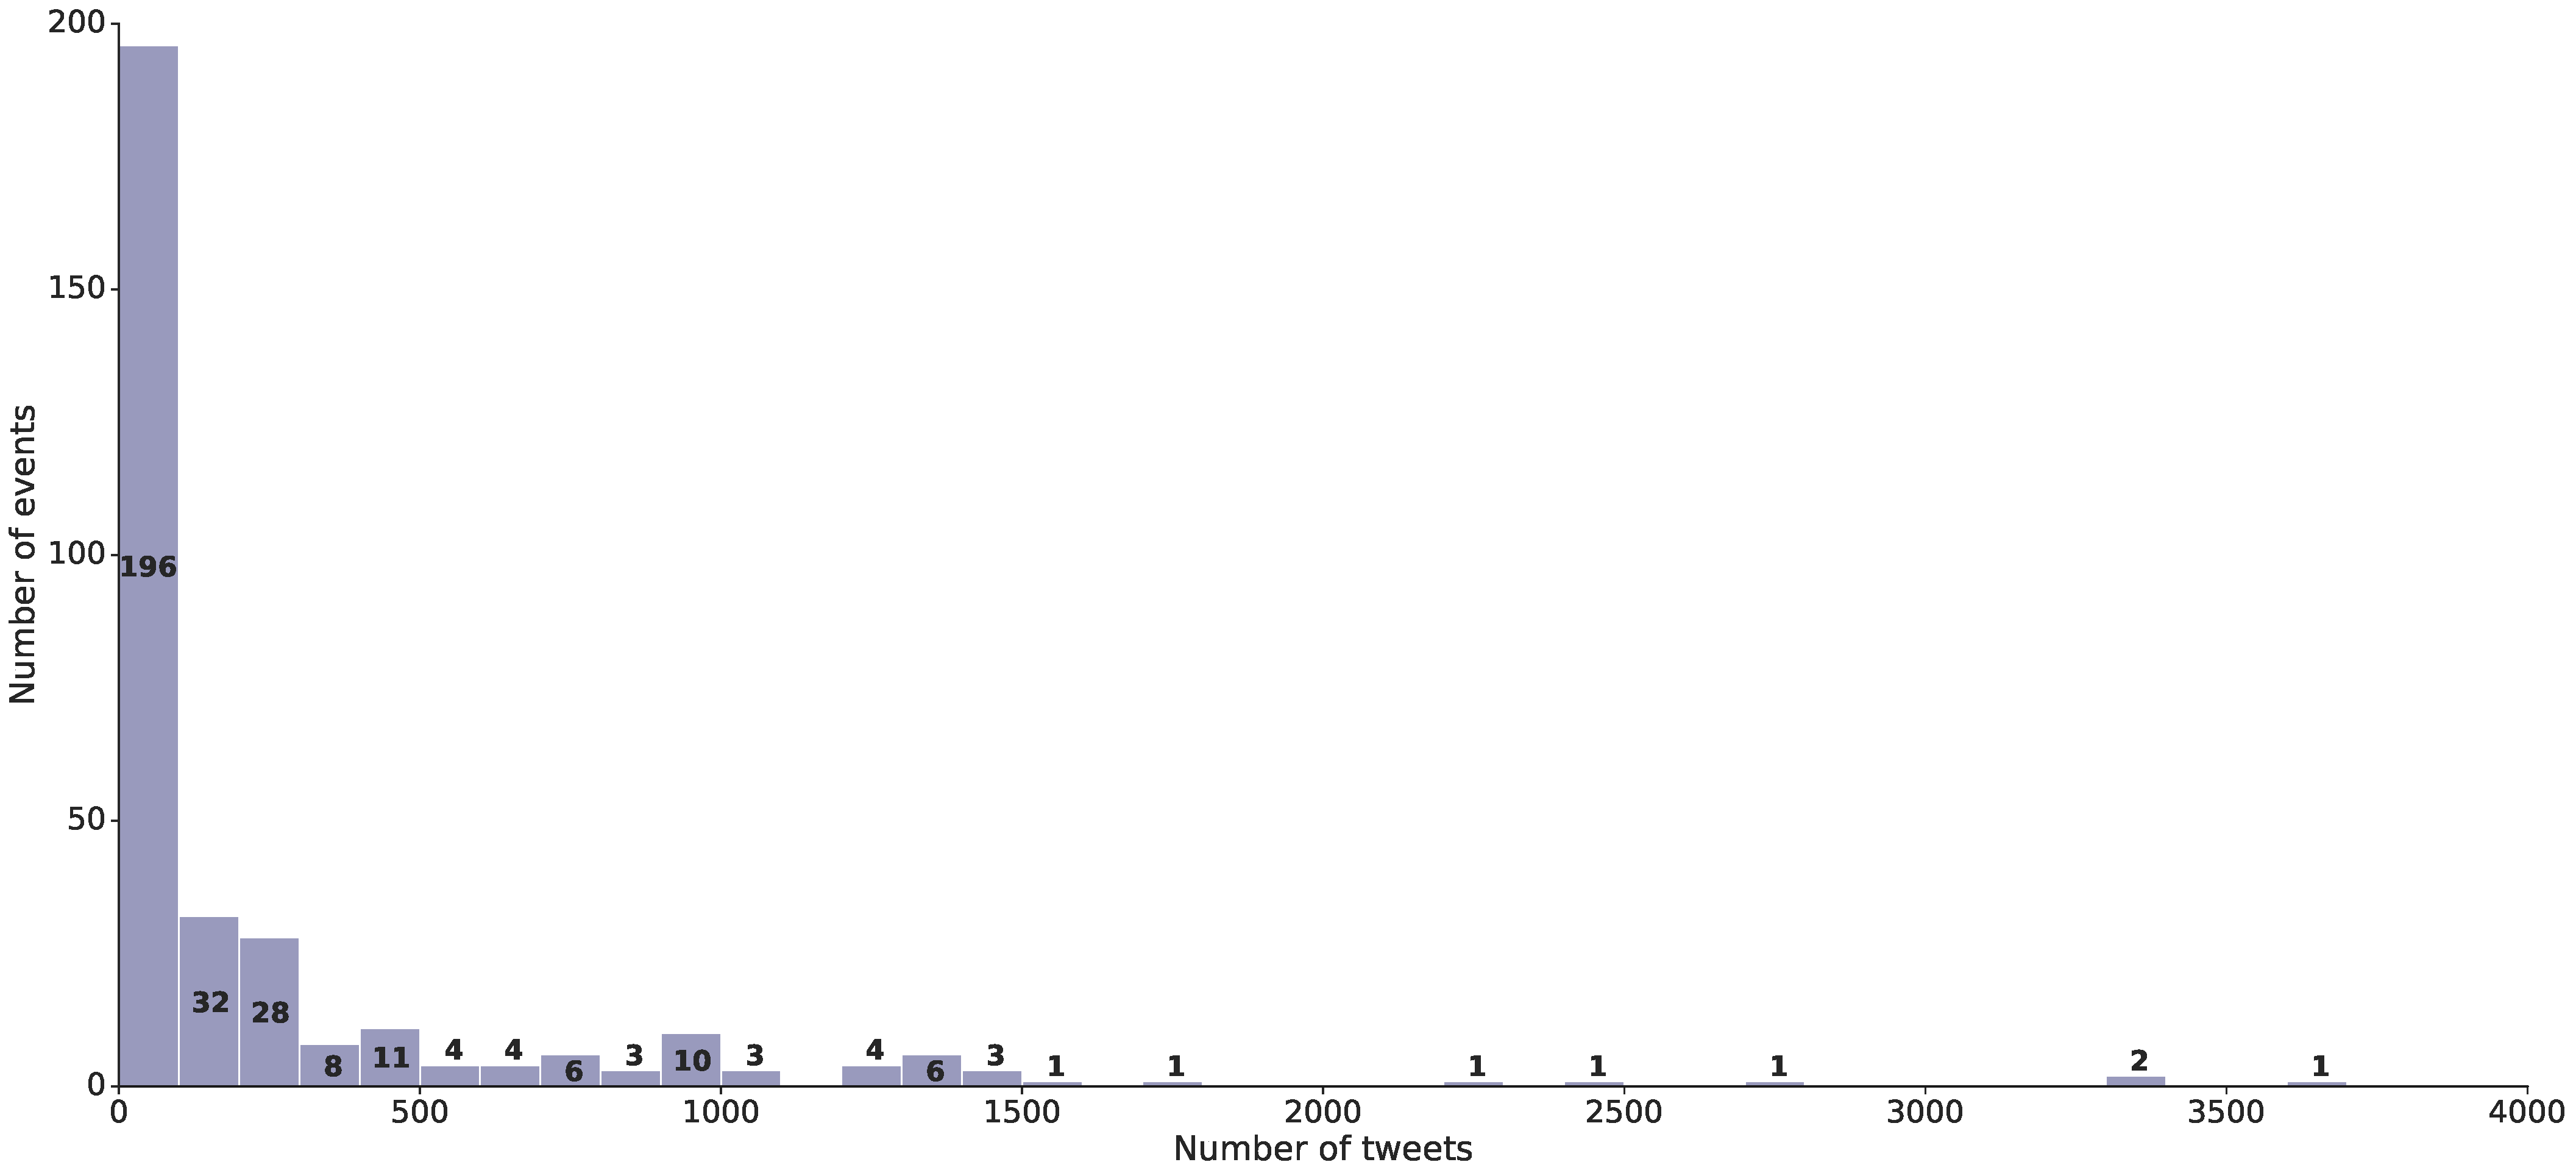
\includegraphics[width=1\textwidth]{figures/HistogramEventsDistribByNbTweets_True.pdf}}
%
%\end{center}
%{\scriptsize 
%
%\textbf{Lecture Note:} 196 events of our corpus contain less than 100  annotated tweets. 32 events of our corpus contain between 100 and 200 annotated tweets, etc.
%}
%\caption{Distribution of the events depending on the number of annotated tweets}
%\label{Figure:HistogramEventsByNbTweets_Related}
%\end{figure}
%%%%%%%%%%%%%%%%%%%%%%%%

%%%%%%%%%%%%%%%%%%%%%%%%%
%\begin{figure}
%\begin{center}
%\makebox[\textwidth][c]{\includegraphics[width=1\textwidth]{figures/Hi%stogramMachineEventsDistribByNbTweets_True.pdf}}
%
%\end{center}
%{\scriptsize 
%
%\textbf{Lecture Note:} 176 events of our corpus contain less than 500 tweets annotated with propagation. 29 events of our corpus contain less than 1000 tweets annotated with propagation, etc.
%}
%\caption{Distribution of the events depending on the number of tweets % annotated with propagation}
%\label{Figure:HistogramMachineEventsByNbTweets_Related}
%\end{figure}
%%%%%%%%%%%%%%%%%%%%%%%%%

To describe the distribution of events across categories we used the classification by the French news agency AFP. AFP dispatches are labeled using the IPTC Information Interchange Model\footnote{\url{https://en.wikipedia.org/wiki/IPTC_Information_Interchange_Model}} Media Topics. This taxonomy is used internationally by numerous media companies to apply metadata to text, images and videos. The distribution of events across the 17 top Media Topics is detailed in Table \ref{Tab:IPTC_cat}. Among the 326 selected events, only 209 were drawn from the AFP and had a label. For the remaining 117 events (from other French press outlets or from Twitter events) we attributed a label manually.

%%%%%%%%%%%%%%%%%%%%%%%%%%%%
\begin{table}
\begin{center}
\makebox[\textwidth][c]{\begin{tabular}{llc}
\toprule
                        English categories &                        French categories &  Number of events \\
\midrule
    arts, culture, entertainment and media &  Arts, culture, divertissement et médias &                12 \\
 disaster, accident and emergency incident &                   Désastres et accidents &                 9 \\
             economy, business and finance &                     Economie et finances &                47 \\
                                 education &                                Education &                 5 \\
                               environment &                            Environnement &                 0 \\
                            human interest &                    Gens animaux insolite &                 8 \\
                   conflict, war and peace &                      Guerres et conflits &                24 \\
                                   weather &                                    Météo &                 0 \\
                    crime, law and justice &                        Police et justice &                71 \\
                                  politics &                                Politique &                53 \\
                       religion and belief &                     Religion et croyance &                 1 \\
                                    health &                                    Santé &                 6 \\
                    science and technology &                   Science et technologie &                 4 \\
                                    labour &                                   Social &                 3 \\
                                   society &                                  Société &                21 \\
                                     sport &                                    Sport &                54 \\
                     lifestyle and leisure &               Vie quotidienne et loisirs &                 8 \\
\bottomrule
\end{tabular}
}
\end{center}
\caption{Distribution of events across the 17 top IPTC Information Interchange Model Media Topics. \label{Tab:IPTC_cat}}
\end{table}
%%%%%%%%%%%%%%%%%%%%%%%%%%%%

\subsection{Intra-event diversity}
The quality of the dataset should also be measured in
terms of variety of the tweets within a given event: what
proportion of the tweets are simply the headline of the
same linked article, for instance? Indeed, the proportion of
tweets containing an url is high among the annotated
tweets (71\%), compared to the entire corpus of 38 million
tweets (36\%). However, due to the design of the
annotation interface (see Section \ref{annotation efficiency}), very few
annotated tweets share the same url. Only 4.6\% of tweets
linked to an event share the same url as another tweet in
the same event.
However, we did not anticipate during annotation that
different urls can link to the same page. After redirection,
9.3\% of tweets share the same page as another tweet in
the same event, but 95\% of pages are shared less than 3
times in a given event.

	\subsection{Annotator agreement}

Annotator agreement is usually measured using Cohen's kappa for two annotators. Here we chose to hire three annotators in order to have an odd number of relevance judgments for each tweet. In the case of several annotators, \citet{randolph_free_2005} recommend to use Fleiss' kappa \citep{fleiss_measuring_1971} in case of ``\textit{fixed marginal distributions}" (annotators know in advance the proportion of cases that should be distributed in each category) and free-marginal multirater kappa \citep{randolph_free_2005} if there is no prior knowledge of the marginal distribution. Indeed, we experienced some odd results using Fleiss' kappa on our corpus, in particular for events with a strong asymmetry between categories (when a large majority of tweets were annotated as ``unrelated" to the event of interest, or the opposite). We hence decided to use free-marginal multirater kappa, which is also the measure used by \citet{mcminn_building_2013}.


If one denote $P_o$ the proportion of overall agreement among annotators, $P_e$ the proportion of agreement expected by chance, free-marginal multirater kappa is expressed as 
$$
\kappa_{free} = \frac{P_o - P_e}{1 - P_e}
$$
with 
$$
P_o = \frac{1}{Nn(n-1)}((\sum_{i=1}^N\sum_{i=j}^kn_{ij}^2)-Nn)
$$
and
$$
P_e = \frac{1}{k}
$$
where $N$ is the total number of cases (here the number of tweets to annotate), $n$ is the number of annotators and $k$ the number of categories (two in our case: \textit{relevant} or \textit{not relevant} to a given event). Its values vary between $-1$ and $1$. A value of $0$ indicates a level of agreement that could have been expected by chance, and a positive value indicates a level of agreement that is better than chance. Negative values indicate worse agreement than expected by chance.


%%%%%%%%%%%%%%%%%%%%%%%%
\begin{figure}
\begin{center}
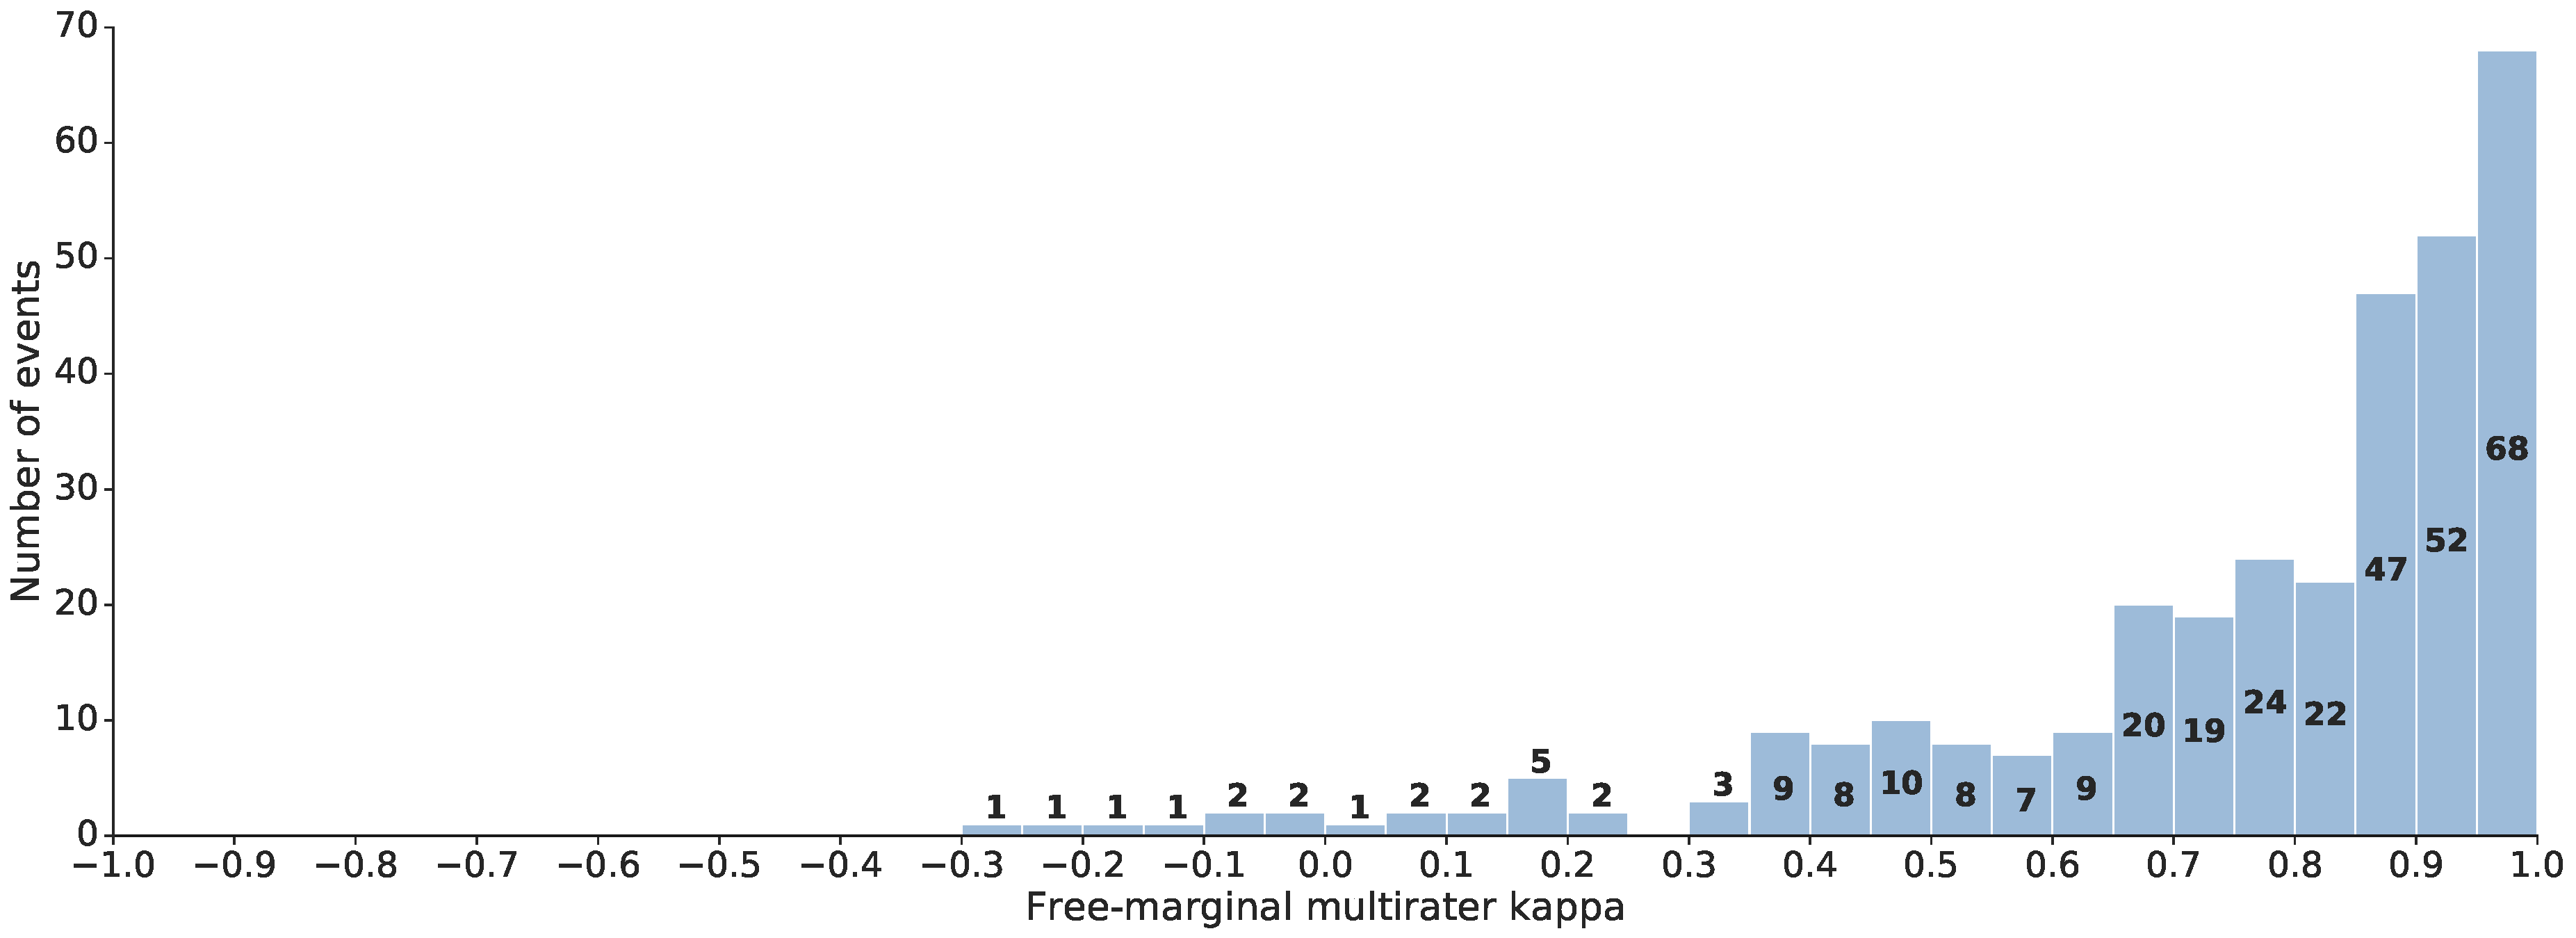
\includegraphics[width=1\textwidth]{figures/HistogramEventsDistributionByKappa.pdf}
\end{center}
{\scriptsize \textbf{Lecture Note:} In our corpus, 121 events have a free-marginal multirater kappa higher than 0.9, 69 events have a free-marginal multirater kappa between 0.8 and 0.9, etc.
}
\caption{Distribution of the events depending on annotators' agreement, measured by free-marginal multirater kappa}
\label{Figure:HistogramEventsByKappa}
\end{figure}
%%%%%%%%%%%%%%%%%%%%%%%%

In our corpus, $\kappa_{free} = 0.79$ which indicates a strong level of agreement among annotators. We also computed the $\kappa_{free}$ value for  each individual event (taking into account all tweets that have been read by annotators while working on this event). Figure \ref{Figure:HistogramEventsByKappa} describes the distribution of events depending on the $\kappa_{free}$. We observe that for some events, the agreement is very low: 8 events have a negative $\kappa_{free}$ value, and 12 events have a $\kappa_{free}$ value between 0 and 0.3.


We asked the annotators to re-read together the events were their agreement was particularly low, in order to understand why they did not annotate tweets the same way. The students admitted some errors in the annotation for 4 of the 17 examined events. For the other events, they explained that they had different views of the events' scope: for example, one article reported the fact that President of Nicaragua Daniel Ortega refused to resign in a context of severe crisis in his country. Two of the annotators included in the event the tweets related to the crisis in Nicaragua. One annotator restricted the event to the statement of Daniel Ortega. Faced with these differences in opinion we could decide to remove from the corpus the tweets were the annotators disagree, or to remove events with a very low kappa. However it seems interesting to see how an algorithm behaves in such borderline cases.


\section{Conclusion}

It is rare in a Machine Learning thesis to devote so much work to the constitution of a corpus: on the contrary, it is rather recommended to work on existing datasets, recognized by the scientific community, and allowing to evaluate  performances on a common benchmark. However, there are several reasons why I took the time to set up a reliable collection method, and spent the summer of 2018 annotating tweets. 

As I showed in Section \ref{state of the art}, publicly accessible tweets corpora for event detection are rare, they are generally quite small and none of them exist in French. I hope that I have been able to contribute through my work to partly remedy this lack, since I published my corpus, with the ids of the 38 million tweets collected during the summer of 2018. Given the number of annotated tweets and the general quality of the annotation (see Section \ref{Evaluation of the created corpus}) it may be useful resource for researchers, especially French-speaking ones.


Working on tweets in French was not only an incentive to build my own corpus, but also to set up my own method of collecting tweets, which I detailed in Section \ref{Tweet collection}, in order to get a sufficient volume of tweets in French. By renouncing to use only the Sample API, which ensures a random distribution of collected tweets, I also had to find methods to evaluate the resulting sample, in order to guarantee its representativity. This work allows me, in the continuation of this thesis, to guarantee the reliability of my analyses.


Finally, the architecture for collecting and indexing tweets, implemented in 2018, has been running continuously until today. It is a tool for INA researchers that will serve even after the end of my thesis. It is currently being used by Nicolas Hervé for a research project on media intensity on the subject of COVID-19  and will hopefully allow many other studies.